% !TEX root = thesis.tex

\chapter{Simulation results}
\label{ch:sim_results}

We present here the results of the simulations performed using the technique presented in the previous Chapter.
We will concentrate on following the journey of the galaxy into the cluster and characterize its evolution depending on the initial mass at the time of injection and its orbit.
Generally, galaxies will undergo some ``phase transitions" which will happen mainly at pericenter passages.
Some of the galaxy will effectively be transformed into Ultra Diffuse Galaxies (as shown in Section~\ref{sec:UDG}), some other will be allowed to briefly be identified as ``jellyfish" (Section~\ref{sec:where_star_formation}).

\begin{sidewaystable}
 \centering
 \footnotesize
 \begin{tabular}{lx{0.8cm}x{1.4cm}x{0.7cm}x{1cm}x{0.8cm}x{0.8cm}x{0.7cm}x{1.9cm}}
\toprule
name & peric. \newline (kpc) & $\log_{10}$(M$_\star$) \newline (M$_\odot$) & $R_e$ \newline (kpc) & $\sigma_\star$ \newline (km/s) & M$_V$ \newline (mag) & M$_{r'}$ \newline (mag) & $n$ & $\bar{\mu}_{e,r'}$ \newline (mag/arcsec$^2$) \\
\midrule
  62 &                        50 &                                        6.50 &                  1.6 &                            6.7 &                 -9.7 &                   -10.1 & 1.1 &                                         28.7 \\
  62 &                       100 &                                        6.57 &                  1.6 &                            8.0 &                 -9.9 &                   -10.2 & 1.0 &                                         28.5 \\
  62 &                       150 &                                        6.59 &                  1.6 &                            9.1 &                 -9.9 &                   -10.2 & 1.4 &                                         28.6 \\
  62 &                       200 &                                        6.59 &                  1.7 &                            8.3 &                -10.0 &                   -10.3 & 1.2 &                                         28.5 \\
  62 &                       300 &                                        6.64 &                  1.7 &                            8.6 &                -10.1 &                   -10.4 & 1.0 &                                         28.2 \\
  71 &                        50 &                                        6.26 &                  6.7 &                           21.6 &                 -9.5 &                    -9.8 & 0.0 &                                         31.8 \\
  71 &                       100 &                                        6.82 &                  6.2 &                            6.5 &                -10.9 &                   -11.2 & 0.5 &                                         30.5 \\
  71 &                       150 &                                        6.79 &                  6.4 &                            0.8 &                -10.7 &                   -11.0 & 0.5 &                                         30.5 \\
  71 &                       200 &                                        6.85 &                  6.9 &                            0.8 &                -11.0 &                   -11.3 & 0.2 &                                         30.4 \\
  71 &                       300 &                                        6.85 &                  7.2 &                            1.8 &                -11.0 &                   -11.4 & 0.2 &                                         29.7 \\
  69 &                        50 &                                        6.81 &                  7.6 &                            1.6 &                -10.6 &                   -11.0 & 0.2 &                                         30.7 \\
  69 &                       100 &                                        7.53 &                  7.1 &                           17.8 &                -12.5 &                   -12.9 & 0.1 &                                         28.4 \\
  69 &                       150 &                                        8.05 &                  4.3 &                           11.6 &                -14.2 &                   -14.4 & 0.3 &                                         26.8 \\
  69 &                       200 &                                        8.34 &                  3.3 &                           18.4 &                -15.0 &                   -15.3 & 1.0 &                                         25.0 \\
  69 &                       300 &                                        8.42 &                  1.8 &                           23.9 &                -15.5 &                   -15.7 & 0.9 &                                         23.5 \\
  68 &                        50 &                                        6.27 &                  8.0 &                            nan &                 -9.1 &                    -9.4 & 0.0 &                                         32.3 \\
  68 &                       100 &                                        6.85 &                  7.3 &                            2.5 &                -10.6 &                   -10.9 & 0.1 &                                         31.2 \\
  68 &                       150 &                                        6.85 &                  7.3 &                            nan &                -10.6 &                   -10.9 & 0.1 &                                         31.2 \\
  68 &                       200 &                                        7.02 &                  7.4 &                            nan &                -11.4 &                   -11.7 & 0.1 &                                         30.0 \\
  68 &                       300 &                                        8.09 &                  3.8 &                           11.5 &                -14.5 &                   -14.8 & 0.8 &                                         26.2 \\
  41 &                        50 &                                        8.93 &                  3.5 &                           16.5 &                -16.2 &                   -16.5 & 1.0 &                                         23.9 \\
  41 &                       100 &                                        8.94 &                  2.5 &                           26.0 &                -16.4 &                   -16.7 & 1.0 &                                         23.0 \\
  41 &                       150 &                                        8.99 &                  1.7 &                           28.5 &                -16.6 &                   -16.8 & 0.8 &                                         22.2 \\
  41 &                       200 &                                        8.97 &                  2.2 &                           29.4 &                -16.6 &                   -16.8 & 0.8 &                                         22.5 \\
  41 &                       300 &                                        9.04 &                  1.8 &                           33.7 &                -17.0 &                   -17.2 & 0.7 &                                         21.8 \\
\bottomrule
\end{tabular}

 \caption{Features of the selected MoRIA galaxies at $z=0$.} \label{tbl:galaxies}
\end{sidewaystable}

In Table \ref{tbl:galaxies} we present the final value of some physical values at the end of the simulations which were performed from $8.5$~Gyr to $\approx 14$~Gyr\footnote{We highlight that each simulation required $\approx 25$ days on average of wall clock runtime on dedicated computing nodes with 32 cores.
}.
Before starting the exposition, we have to introduce a couple of concepts which revealed particularly useful in the analysis and allowed for better comparison among the different MoRIA galaxies and the orbits introduced above.

\paragraph*{Radial period}
Pericenter passages, as explained in the following, are important moments for the life of the simulated dwarf.
In order to compare different orbits, we normalise the simulation time by the orbital radial period $T_r$, \ie{} the time between two pericenter passages, \citep[p.~146]{BinneyTremaine2008}:
\begin{equation}
    T_r = 2 \int^{r_a}_{r_p} \frac{\dd r}{\sqrt{2\left[E-\Phi(r) \right] - J^2/r^2}}
    \label{eq:radial_period}
\end{equation}
where $r_p, r_a$ are the pericenter and apocenter distance respectively, $E$ and $J$ the orbital energy and angular momentum per unit mass, $\Phi(r)$ the potential at radius $r$ of the NFW halo around which the galaxy is orbiting.

By defining the time of pericenter passage as $t_p: r(t_p) = r_p$, we can introduce the normalized time:
\begin{equation}
  \label{eq:tau}
\tau = \frac{t-t_p}{T_r},
\end{equation}
which is~$0$ or $1$ for first or second pericenters respectively,~and~$0.5$ for apocenter passages.

% We begin with following one galaxy in its journey around the cluster.
In the following we will compare the effects of orbit and initial mass using the set of 25 simulations we have carried out.


\paragraph*{Tidal radius}
As we shall see, the cluster gravitational potential is able to strip material from the galaxy. Some of the simulations, depending on the orbit they are on, will become gravitationally unbound dominated by the cluster potential.
We chose to define the event of becoming unbound using the condition on the tidal radius \cite{King1962}: namely when it becomes smaller than the effective radius.
This criterion tests whether the stellar body of the galaxy would become unbound and dissolved, which is what an observer would consider for the detection of a ``galaxy''.
Physically, also this implies that orbits of the stars in the outskirts of the galaxy are influenced by the cluster potential more than they are by the galactic halo potential.
Tidal radius $r_t$ is computed as follows:
\begin{equation}
r_t = r \sqrt[3]{\frac{M_g}{M_c(r) (3+e)}},
\label{eq:tidal_radius}
\end{equation}
where $e = (r_a - r_p) / (r_a + r_p)$ is the eccentricity of the orbit computed, $r_a$, $r_p$ the apocenter and pericenter radii respectively; $M_c(r)$ is the enclosed cluster mass at radius $r$, and $M_g$ the instantaneous total mass of the galaxy.
As a convention we measure the galaxy mass as the total mass (baryonic and dark matter) within $10$~kpc from the center of the galaxy.

In Figure \ref{fig:tidal_radius} we show an example of $r_t$ evolution along the orbit.
We define a galaxy to become unbound when the condition
\begin{equation}
    R_e > r_t
\label{eq:tidal_radius_condition}
\end{equation}
first occurs.
%Galaxies on a radial orbits will undergo disruption more easily.
\begin{figure}
\centering
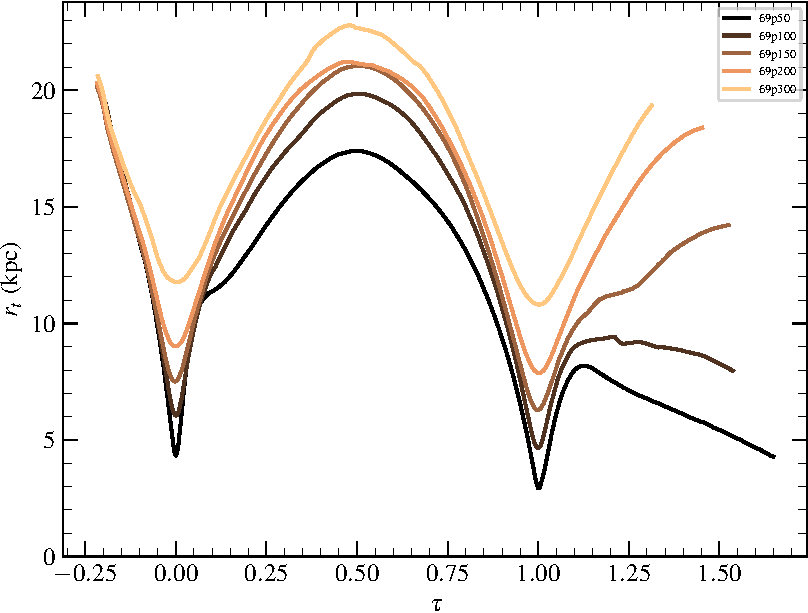
\includegraphics[width=\textwidth]{14.0_tidal_radius.pdf}
\caption{Evolution of the tidal radius for the simulations ID 69.}
\label{fig:tidal_radius}
\end{figure}

\section{Becoming an Ultra Diffuse Galaxy (UDG)}
\label{sec:UDG}

Faint Low Surface Brightness (LSB) galaxies have been detected in galaxy clusters since the 1980s \citep[e.g.][]{Sandage1984}.
% See Wittmann  https://www2.mpia-hd.mpg.de/homes/galClusters_2017/slides/Ringberg2017_presentation_Wittmann.pdf

% Wittmann2017 studies LSB in Perseus
LSB galaxies are defined as having \citep{Venhola2017}:
\begin{equation}
\begin{cases}
 \mu_{0,r'} > 23 \mbox{ mag/arcsec}^2\\
 M_{r'} > -19
\end{cases}
\end{equation}

In 2015 \citet{VanDokkum2015} introduced a size criterion to distinguish between LSB galaxies and more compact `normal' dwarfs \citep{Sales2021}:
UDG are therefore defined as large ($R_e > 1.5$~kpc) low surface brightness galaxies.
%($\bar\mu_{r',e} > 24$~mag/arcsec$^2$).

The majority of studies indicate that they have the properties of large dwarf galaxies \citep{Sandage1984, Roman2017, Venhola2017, Saifollahi2021}.
Three main mechanisms are hypothesized as possible formation scenarios for UDGs:
\begin{itemize}
  \item dwarf galaxies which undergo strong tidal stripping \citep{Venhola2017, Carleton2018, Rong2020a};
  \item gas outflows driven by stellar feedback with extended dark-matter halo and faint and diffuse stellar component \citep{DiCintio2017, ManceraPina2019},
  \item or failed $L_\star$ galaxies\footnote{An $L_\star$ galaxy has a luminosity equal to the characteristic luminosity of the Schechter luminosity function \citep{Press1974}.
  Its value is about $L_\star \approx 3\times10^{11}L_\odot$, \cf{}  \citet{Cooray2005}.}
in high mass dark halos with ceased star formation in the early universe.
\end{itemize}
Some UDGs have earlier been identified as disrupted early-type galaxies.
\citet{Koch2012} is indeed able to reproduce a typical S-shape tidal tailed UDG HCC-087 in the Hydra I cluster via simulations considering only the cluster potential.
It is worth noting that in their simulations they find an orientation of the tidal tails perpendicular to the orbit, which will be important in Chapter~\ref{ch:ngc1427a}.

The cluster alignment of UDGs is also a quantity which in various cluster has been measured.
The signs of elongation, which will be discussed further in~Section \ref{sec:3d_ellipticity}, have been used to infer the origin of UDGs.
In the Coma and Abell 1314 clusters \citep{Yagi2016, ManceraPina2019} UDGs are preferably aligned towards the cluster center.
This suggesting that they may be the products of strong tidal interaction with the cluster.
In the Fornax cluster, however, the low statistics do not allow for a conclusive analysis.
On the other hand at least two of the detected UDGs in Fornax show sign of elongation towards a nearby dwarf galaxy \citep[with $M_{r'} > -19$~mag, see][]{Venhola2017}.
As shown by \citet{Rong2020}, for the Abell 2634 cluster, the minor axes of UDGs tend to be aligned with the major axis of the central dominant galaxy.
It is implied therefore that, in this case, UDGs are possibly very recent infallers, still retaining signs of their primordial alignment in the closest large-scale filament they came from.

\paragraph{UDGs in Fornax}
\citet{Venhola2017} found nine UDGs candidates within an area of $4$~deg$^2$ centered in NGC1399.
The ratio of UDGs to dwarf galaxies in Fornax is consistent with that in the Coma and Virgo clusters.
Also, the number of UDGs within the virial radius are correlated with the virial mass of the cluster.
In the size-magnitude parameter space, UDGs in Coma form a continuous distribution, whereas in Fornax two of them are  remarkably luminous, and can be considered as outliers.
Also, UDGs in Fornax are among the more luminous galaxies and their colour correlates with surface brightness, becoming redder with increasing surface brightness.
They follow the same color-magnitude relation as dwarfs, which suggests a link between UDGs and dwarf galaxies  (\cf{} Section~\ref{sec:CM}).
% As expected, Sérsic index is around $1$
As opposed to the ones in the Coma cluster, their alignment with respect to the cluster potential is not evident: in Coma UDGs are oriented towards the cluster center, whereas in Fornax, as mentioned above, there's no correlation.
It is interesting to note that larger UDGs are more elongated as opposed to UDGs in Coma.

\subsection{Size and magnitudes}
Once approaching the pericenter, energy is transferred to the galaxy, according to the virial theorem.
%According to the virial theorem %predicts that by adding energy to a galaxy, it will increase its radius:
%once approaching the pericenter, energy is transferred to the galaxy:
Stars thus migrate to more energetic and hence wider orbits.
In addition, mass is lost due to tides, making the gravitational well even more shallow and leading to potentially large increases in radius.
We compute the 3D effective radius shown in Figure~\ref{fig:r_eff}.
This radius is independent of the orientation of the galaxy, and it has been computed as the radius of the sphere which contains half the total luminosity of the galaxy.
Tidal heating affects the size of the galaxies as they pass near the cluster center, with low mass galaxies affected most.

% We compare the resulting effective radius in simulations with the ones not taking into account the gas inside the cluster, Figure~\ref{fig:r_eff_no_gas}.

\begin{figure}[ht]
\centering
\includegraphics[width=\textwidth]{{00.0_fig_3dreff_time}.pdf}
\caption{3d effective radius evolution with time normalised with the radial period of the orbit. Curves are smoothed using a rolling average of 0.2~Gyr and are truncated as soon as condition \eqref{eq:tidal_radius_condition} is verified.}
\label{fig:r_eff}
\end{figure}

% NOTE See whether to put this plot
% \begin{figure}
% \centering
% \includegraphics[width=\columnwidth]{{00.2_3dreff_gas_no_gas_last_Re_color}.pdf}
% \caption{Relative change in effective radius between simulations with tides only ($R^{3D}_{e, ng}$), and cluster infall simulations with RPS ($R^{3D}_e$) at redshift $z=0$.}
% \label{fig:r_eff_no_gas}
% \end{figure}
% \subsection{Dark halo concentration}
% Between two pericenters material falls back in the galaxy, see Figure~\ref{fig:dm_halo}.

% NOTE maybe it is better to compare a sphere of 2 kpc with one of 10 kpc, and not comparing spheres with cubes.

% \begin{figure}
% \centering
% \includegraphics[width=0.9\columnwidth]{{12.0_dm_ratio}.pdf}
% \caption{Ratio between dark-matter mass contained in a sphere of $10$ kpc radius $M_h^{c}$ and the total dark-matter mass contained in the moving box, $M_h^{tot}$.}
% \label{fig:dm_halo}
% \end{figure}

% \subsection{Stellar metallicity gradients}

\subsection{$M_h/M_\star$}
We computed the stellar and dark-matter mass inside a sphere of radius $10$~kpc centered on the dwarf and the masses inside the entire moving box.
While stars gets formed around pericenter passages, dark matter instead is pulled out by tidal forces who elongate the halo, effectively stripping dark-matter particles out of the moving box of our simulation setup.
This is confirmed for example by comparing the amount of dark matter inside the $10$~kpc region around the dwarf with the whole dark matter present inside the moving box.
As shown in Figure \ref{fig:dm_center_inflow}, there is an inflow of dark matter towards the dwarf galaxy due to tidal squeezing and compression, soon followed by an expansion, resulting in a dearth of dark matter after the first pericenter passage. % NOTE possibly do dark matter profile around pericenter?
For very radial orbits, around first infall, central halo mass increases more than the stellar mass created by the starburst, Figure~\ref{fig:m_halo_m_star}.

\begin{figure}
\centering
\includegraphics{{12.5_dm_ratio_one_sim}.pdf}
\caption{Relative amount of central dark matter $M_{h}^c$
(computed as the mass inside a sphere of 10~kpc of radius around the galaxy)
with respect to the dark matter in the simulation box ($M_{h}^{tot}$) for sim ID 69.
Colours indicate the pericenter distances of the different orbits.
}
\label{fig:dm_center_inflow}
\end{figure}
\begin{figure}
\centering
\includegraphics[height=0.95\textheight]{{12.1_m_halo_m_star}.pdf}
% \includegraphics[width=0.75\columnwidth]{{12.1_m_halo_m_star}.pdf}
\caption{$M_h/M_\star$ around first infall. Halo and stellar mass are computed in a $10$~kpc sphere around the galaxy.
The different orbits with the respective pericenters are color coded as shown in the legend.}
\label{fig:m_halo_m_star}
\end{figure}

\subsection{Central stellar velocity dispersion}
We measured the central (within $250$ pc) stellar velocity dispersion for all the simulations on their orbits, as shown in Figure~\ref{fig:sigma}.
\begin{figure}[ht]
\centering
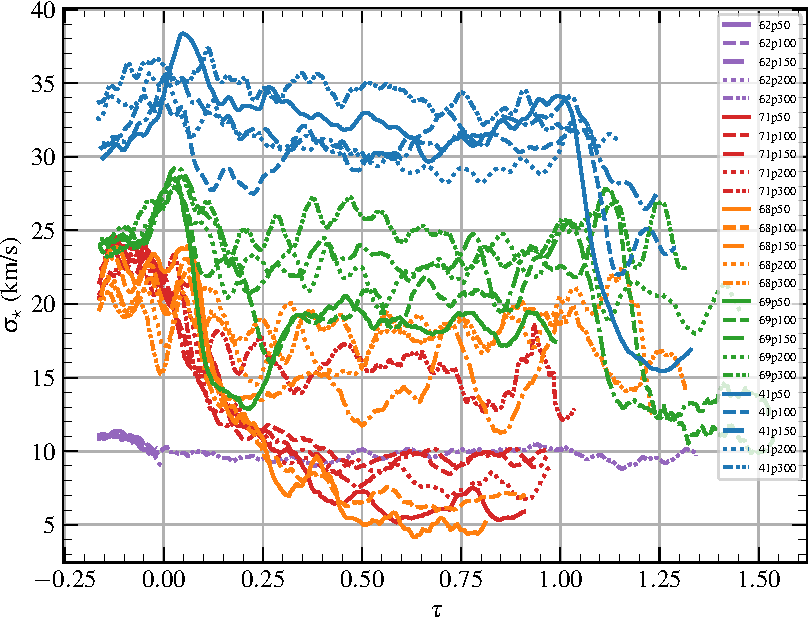
\includegraphics[width=\textwidth]{01.0_fig_sigma_time.pdf}
\caption{The evolution as a function of time (normalized with orbital radial period) of the
line-of-sight velocity dispersion of star particles within a $250$~pc from the galactic center.
Curves are smoothed using a rolling average of 0.2~Gyr.
}
\label{fig:sigma}
\end{figure}
For simplicity we adopted a common point of view for all the orbits, and the line-of-sight velocity dispersion is computed assuming the observer laying in the orbital plane.
As tidal interactions stir the particles in the center of the galaxies, at the pericenter passages a bump in the central velocity dispersion (denoted by~$\sigma$) can be seen.
The following temporary decrease in central velocity dispersion can be linked to the variations of~$M_h/M_\star$.
Tidal squeezing increase~$\sigma$ while subsequent mass loss can dramatically lower it.

\begin{figure}[ht]
\centering
%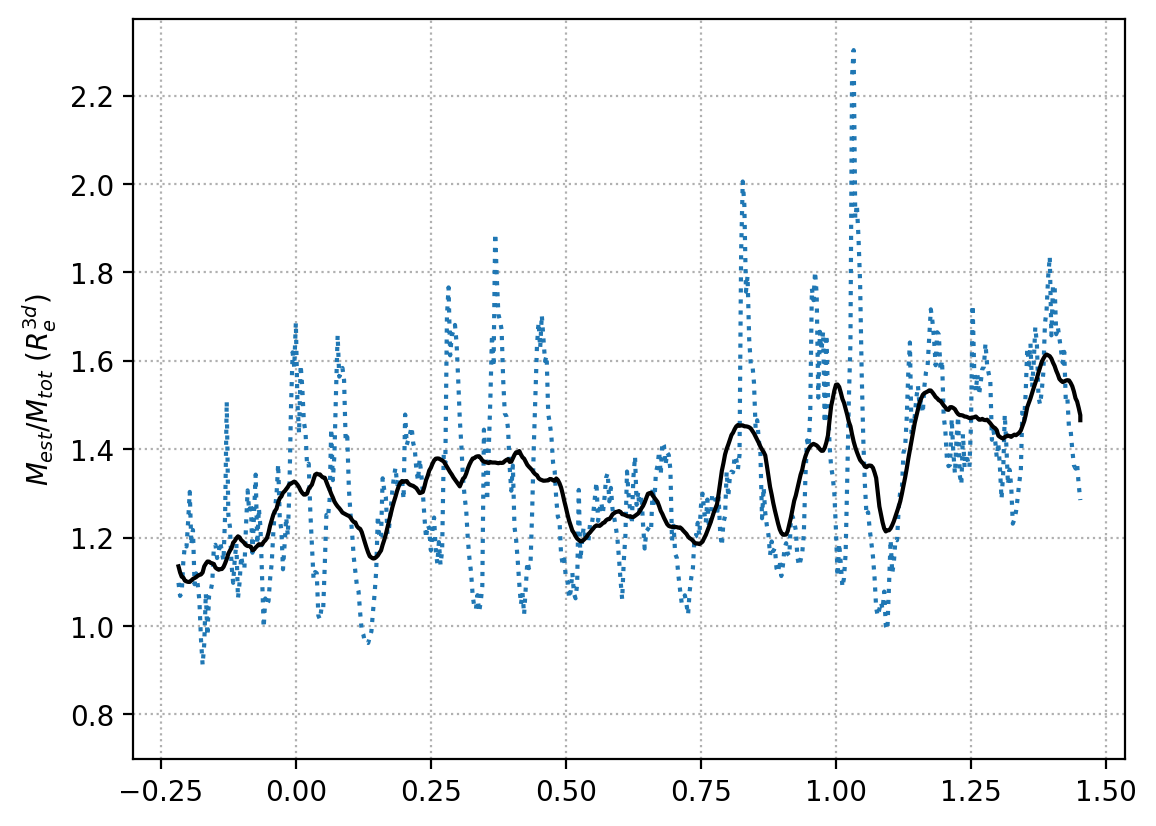
\includegraphics[width=\textwidth]{wolf_m_est_ratio69p200.png}
%\caption{In blue the estimated mass from velocity dispersion with equation \eqref{eq:wolf} relative to the total mass within an effective radius computed from simulation particles,
%for simulation ID 69 on an orbit with 200~kpc pericenter.
%In black the local rolling average with a window of 30 snapshots.
%}
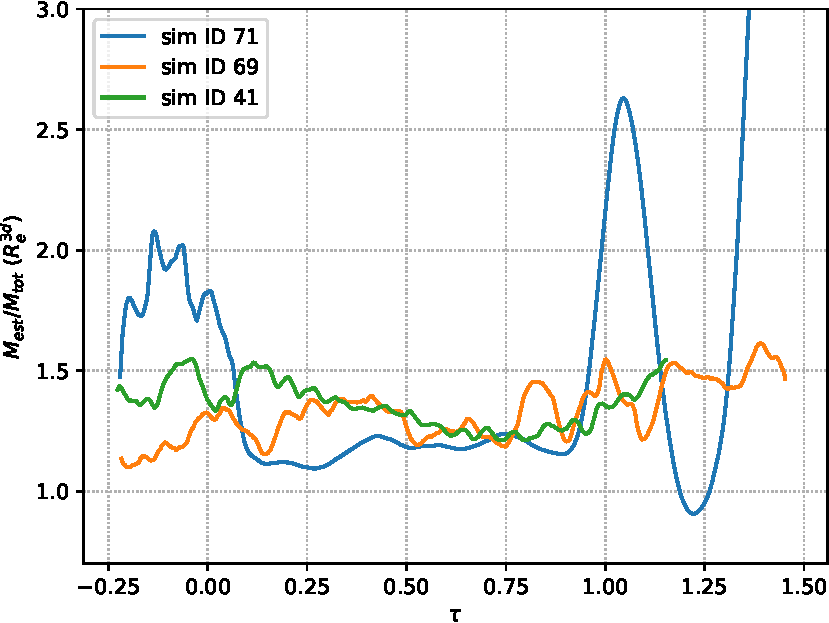
\includegraphics[width=\textwidth]{mass_sigma_multi_sim.pdf}
\caption{The estimated mass from velocity dispersion with equation \eqref{eq:wolf} relative to the total mass within an effective radius computed from simulation particles,
for simulation ID 69, 71, 41 on an orbit with 200~kpc pericenter.
Dashed line indicates unbound snapshots (\ie{} for which the condition \eqref{eq:tidal_radius_condition} is not verified anymore).
}
\label{fig:wolf}
\end{figure}

We checked the dynamical mass estimation which can be computed from the velocity dispersion using the \citet{Wolf2010} relation:
\begin{equation}
\label{eq:wolf}
M^{dyn}_{est} = \dfrac{3}{G} \sigma_e^2 R_e,
\end{equation}
where $\sigma_e$ is the luminosity-weighted line-of-sight velocity dispersion within an effective radius~$R_e$,
and $G$ the gravitational constant.
The result three representative simulations is shown in Figure~\ref{fig:wolf}.
For the low mass galaxy (simulation ID 71), the estimation is not reliable anymore as soon as the galaxy becomes unbound (dashed line in Figure~\ref{fig:wolf}), \ie{} the condition \eqref{eq:tidal_radius_condition} does not hold anymore.
The method of equation \eqref{eq:wolf} overestimates the mass by $\approx20-50\%$ depending on the orbital phase.
Given the simplicity of the method, this relation between the estimated value and the ground truth mass is quite remarkable.
From this, we can learn that despite some conditions required for the application of the method ---~such as equilibrium and sphericity~--- not being fulfilled, the dark-matter content estimates with this method are reliable within an acceptable relative range.

% NOTE The anisotropy parameter $\beta$ can be taken into account

% \citep{Danieli2019} Low dark matter galaxies.

\subsection{3D ellipticity} \label{sec:3d_ellipticity}
We computed the 3D ellipticity of the stellar component of the galaxies using the Principal Components Analysis \citep[PCA, ][]{Pearson1901}.
The first principal component $\vect{w}_2$ is the direction of highest elongation (largest variance of the star particle positions) computed via PCA\footnote{
$\vect{w}_2$ is defined as the eigenvector corresponding to the largest eigenvalue of the covariance matrix $C = \frac 1 {(N-1)} AA^T$, where $A$ is the matrix of the position of the star particles centered on the barycenter of the stars, and $N$ the number of particles.}.

Around pericenter the main elongation direction of the ellipsoid ($\vect w_2$) is aligned with the cluster center; then it undergoes a ``slingshot effect" after pericenter and it aligns with the cluster center also around apocenter before falling back in. This behaviour is shown in Figure~\ref{fig:pca}.
Around the second pericenter passage, for radial orbits, the galaxy ends up being dispersed and not anymore gravitationally bound.

In Figure~\ref{fig:pca_angle_r}, we show quantitatively the relative orientation between $\vect{w}_2$ and the clustercentric direction for simulation ID 69.
Around both pericenter passages the galaxy becomes aligned with the cluster center.
The maximum alignment is obtained at a delayed time depending on the radiality of the orbit.
Also, for all the orbits, the galaxy shows an aligment of an angle $<30$~deg if the orbital phase lays within a quarter of the radial period soon after pericenter, \ie{} $\tau \in [0, 0.25] \cup{} [1, 1.25]$.
% This translates in a time interval of , , depending on the orbit.
Except for the orbit with 100~kpc pericenter, it is possible to see how at apocenter the main elongation is perpendicular to the cluster center. % For this orbit it is likely that due to a swap between

Analogously, we can compute the angle between the elongation direction and the instantaneous velocity along the orbit.
As shown in Figure~\ref{fig:pca_angle_v}, because of the high relative speed and the delay in the formation of tidal tails, around pericenter passages the angle beteen $\vect{w}_2$ varies significantly.
Interestingly, just before the pericenters, velocity is almost perpendicular to the direction of elongation.
At the same time, stripping intensity is at its peak (see Figure~\ref{fig:r_rps}) creating a gaseous tail aligned with the instantaneous velocity of the galaxy.
This misalignement between the tails is shown in detail in Chapter~\ref{ch:ngc1427a} and can be used to infer orbital properties of observed galaxies in cluster.

\begin{figure}
\centering
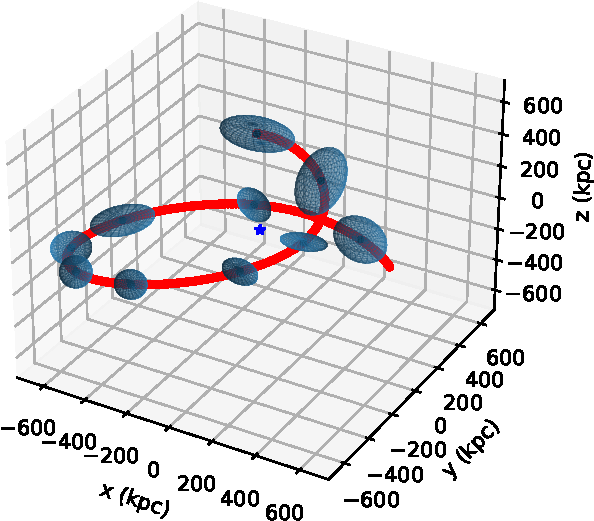
\includegraphics[width=\textwidth]{3d_qualitative_69p200.pdf}
\caption{Qualitative overview of the principal components ellipsoids for the stellar particle positions of the galaxy along its orbit.
In red the orbit of the galaxy, ID 69 with pericenter of 200 kpc.}
\label{fig:pca}
\end{figure}

\begin{figure}
\centering
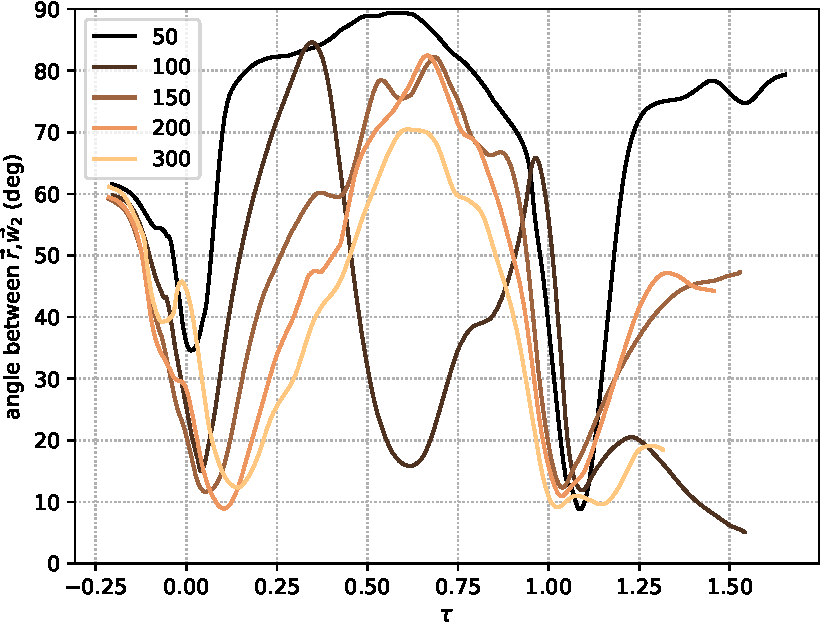
\includegraphics[width=0.8\textwidth]{69_r_angle.pdf}
\caption{Angle between the largest principal component $\vect{w}_2$ and the direction to the cluster center for simulation ID 69. The galaxy shows an aligment of an angle $<30$~deg soon after pericenter passages \ie{} if the orbital phase $\tau \in [0, 0.25] \cup{} [1, 1.25]$.}
\label{fig:pca_angle_r}
\end{figure}
\begin{figure}
\centering
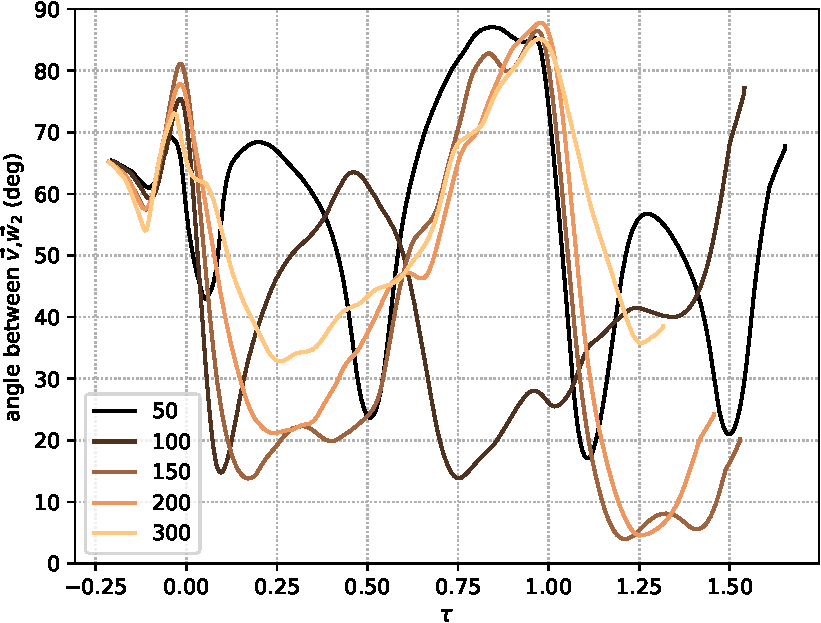
\includegraphics[width=0.8\textwidth]{69_v_angle.pdf}
\caption{Angle between the largest principal component $\vect{w}_2$ and the instantaneous velocity for simulation ID 69.}
\label{fig:pca_angle_v}
\end{figure}

\section{Star formation} \label{sec:where_star_formation}
As shown in the previous section, elongation of material around low clustercentric distances may create grooves in the potential well which lead to angular-momentum transport.
In turn this helps funneling gas towards the center of the galaxy which is squeezed and can cool to create stars.
% TODO non gas run may isolate the role of star formation.
% Ram pressure stripping and tidal interaction can funnel gas into the inner part of the galaxy.
The total content of star forming gas is shown in cyan in Figure~\ref{fig:cold_gas} alongside with the specific star formation rate.
It is interesting to note that for an intermediate mass dwarf, the stripping phenomenon is highly nonlinear.
For example for simulation ID 68, as shown in the corresponding panel in Figure \ref{fig:cold_gas}, the relatively small change of orbit from 150~kpc pericenter to 100~kpc makes the dwarf completely stripped of its reservoir of cold gas.
Due to the stripping, after a burst, star formation stops.
\begin{figure}
\centering
\includegraphics[height=0.95\textheight]{{12.6_sfr_cold_gas}.pdf}
\caption{Specific Star Formation Rate (sSFR) and cold gas (T<$15000$~K) evolution on different orbits.
Different orbits for each galaxy are indicated with shades of brown for the sSFR, and with shades of cyan for the cold gas.}
\label{fig:cold_gas}
\end{figure}

% \citet{Tonnesen2012} argue that pressure in the cluster has a primary role in regulating SF as opposed to the strength of ram pressure.
% NOTE compute cluster gas pressure corresponding to SFR peaks.

% NOTE \citet{Hausammann2019} introduce the parameter $\beta$ defined as the ratio between the ram pressure and the thermal pressure as factor influencing the SF


\subsection{Where do stars form?}
\begin{figure}
\centering
\begin{subfigure}[t]{0.83\textwidth}
\centering
\caption{Simulation ID 71}
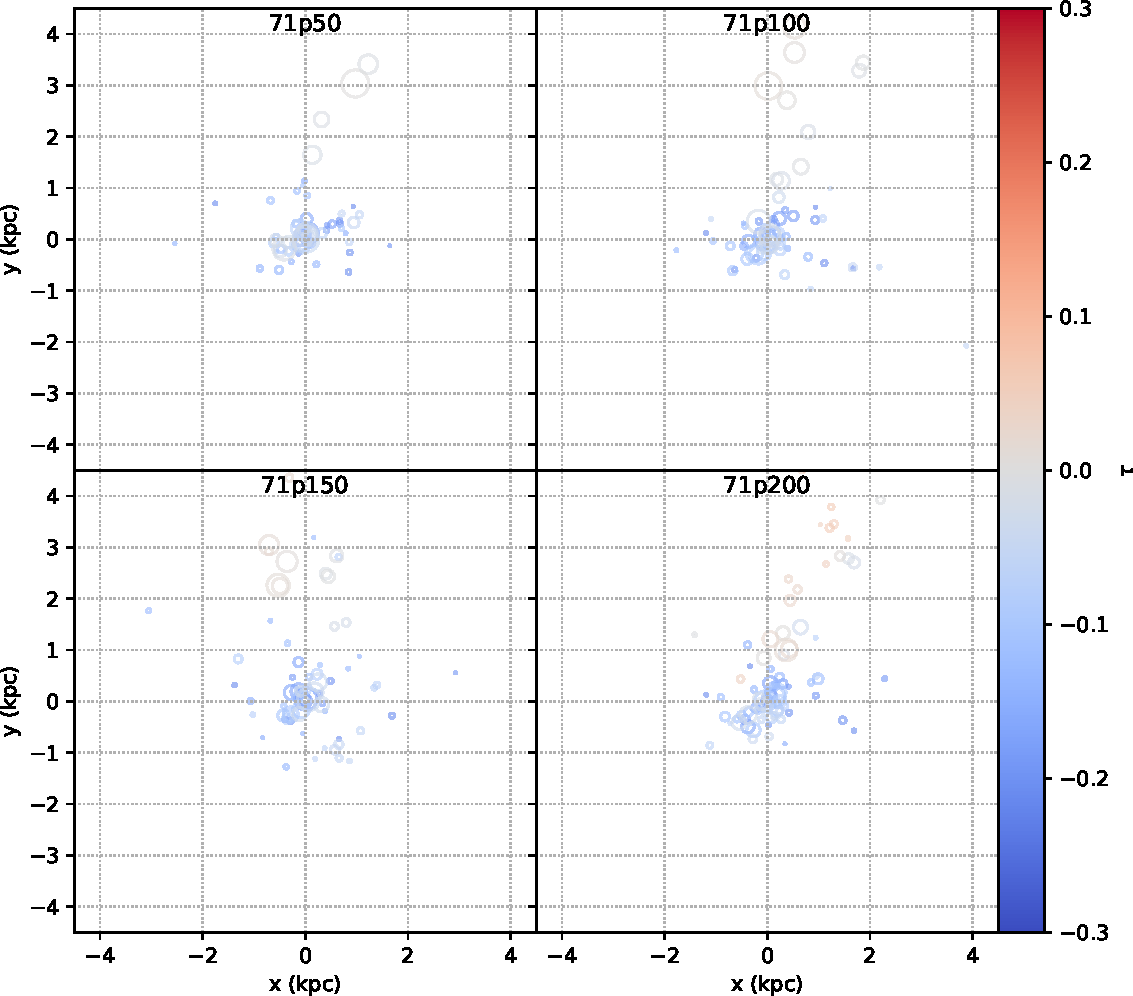
\includegraphics[width=\textwidth]{StarFormationLocation_new71_hollow.pdf}
\end{subfigure}\\%[1.5ex]
\begin{subfigure}[t]{0.83\textwidth}
\centering
\caption{Simulation ID 69}
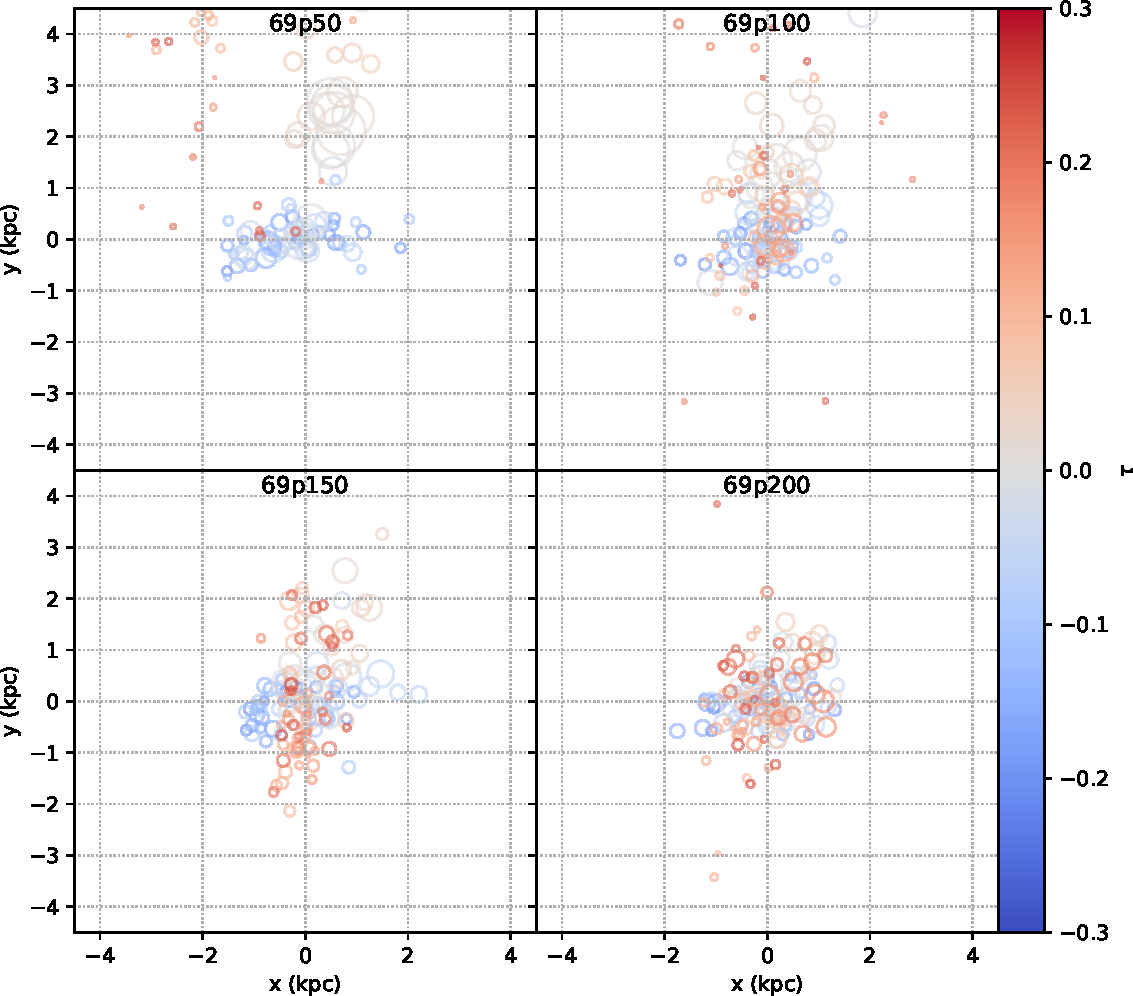
\includegraphics[width=\textwidth]{StarFormationLocation_new69_hollow.pdf}
\end{subfigure}
\phantomcaption
\label{fig:sf_location}
\end{figure}
\begin{figure}[ht]
\centering
\ContinuedFloat % continue from previous page
\begin{subfigure}{0.83\textwidth}
\caption{Simulation ID 41}
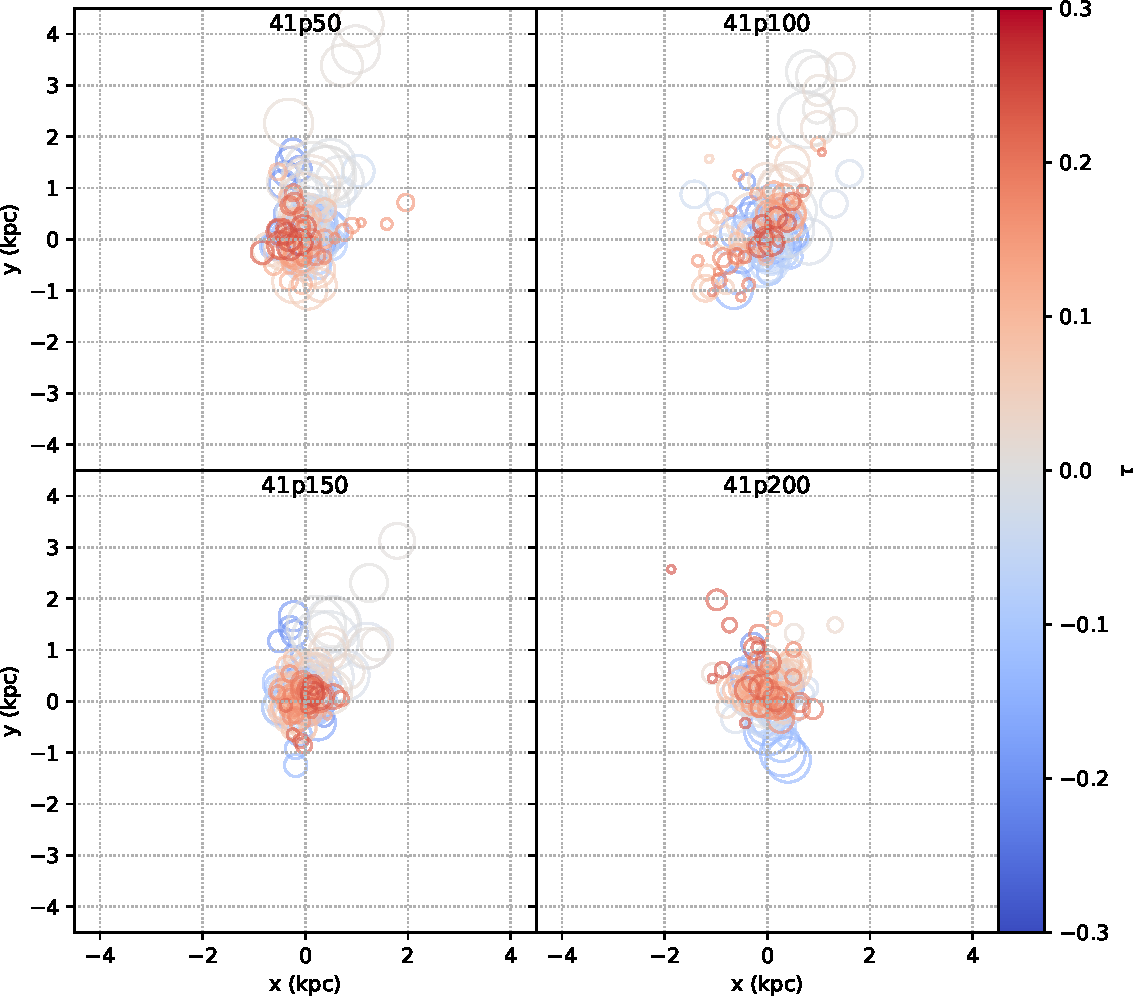
\includegraphics[width=\textwidth]{StarFormationLocation_new41_hollow.pdf}
\end{subfigure}
\caption{Star formation location around first pericenter passage for simulation ID 71, 69 and~41.
Each subpanel corresponds to a different pericenter.
The markers corresponds to the barycenter of the positions of the newly formed stars in each snapshot and are colored according to the distance in time from pericenter normalized with the radial period.
The size of the markers is proportional to the number of stars born between the current snapshot and the previous one.}
\end{figure}
In Figure \ref{fig:sf_location} we show the average position of the star forming particles for each simulation snapshot.
The galaxy is moving in the $-y$ direction (the direction of the instantaneous velocity, see \refsec{sec:MovingBox}) around pericenter.
For each simulation snapshot the number of new stars with respect to the previous snapshot ($10$~Myr before) is counted and their average position in the $xy$ plane is plotted\footnote{
We could have computed the star formation rate from the last galaxy snapshot at $z=0$, reading the time of formation of the star particles.
This is the common approach %\citep[e.g.][]{Hausammann2019}
when computing star formation histories of galaxies, and it is observationally motivated.
In fact the star formation history of an observed galaxy is inferred from the photometry and spectrum of the detected starlight.

However, the large amount of star particles lost during the orbit, leads to a large underestimation (of a maximum of 30\% for the most recent bins especially on low mass galaxies on radial orbits) of what has actually happened during the galaxy journey around the cluster.
The method of counting individual star particles newly born is therefore employed.
The choice of a high frequency snapshot cadence plays a fundamental role to this end.
}.
In this projection the instantaneous velocity of the galaxy is always directed towards the $-y$ axis.
The ram pressure is therefore pushing in the vertically upwards direction in these diagrams, causing gas to be stripped and stars to be formed in the upper part of the panels.

In correspondence of pericenter passage an intense star formation activity is registered in the gaseous tail.
These galaxies can therefore be defined \emph{jellyfish} galaxies \citep{Ebeling2013}:
the term applies, in fact, to galaxies with star formation activity within the stripped gaseous tails.
Star formation flickers on and off inside the gaseous tails as gas clumps are able to cool, condense and create stars.
This result supports the idea that the jellyfish phenomenon is a relatively short transitory phase of the galaxy along its orbit.

In the three panels of Figure~\ref{fig:sf_location}, three representative galaxies are shown in increasing order of mass.
For the least massive galaxy (simulation ID 71), as confirmed in Figure~\ref{fig:cold_gas}, no stars are formed after pericenter (red markers) because the cold gas is completely stripped by ram-pressure.
However, during the stripping phase new star particles appear in the gaseous tail.
For the intermediate mass galaxy (simulation ID 69), in the radial orbits, the behaviour is similar to simulation ID 71.
Also, a front of newly born star is formed in the center (see panel $69$p$50$) as the gas is compressed and pushed upwards.
For the more circular orbits, stars are continuously formed in the center.
This is a behaviour similar to the most massive galaxy, simulation ID 41, where clumps of gas are detached only in radial orbits.
For the 200 kpc orbit ($41$p$200$) stars are even born in front of the galaxy meaning that for a galaxy so massive a layer of star forming gas is not displaced by ram-pressure even at the leading edge of the galaxy.

\section{Colour Magnitude} \label{sec:CM}
The catalogue of dwarf galaxies in the Fornax cluster, prepared by \citet{Venhola2019}, can be used to directly compare our results with observations.
We build the Color-Magnitude (C-M) diagram with all the simulation snapshots, after computing their SDSS-band colors and magnitude.
We then superimposed it on the results of the observations: as shown in Figure~\ref{fig:g-r} there is a good agreement between the catalogue values and our simulations.
In Fornax, the slopes of the C-M relations are different between the morphologically selected late-type and early-type galaxies.
The relation for the former is rather flat, meaning that the color is not correlated with magnitude, whereas the early-types become redder with increasing total luminosity.

In our simulations, the simulated dwarf galaxies tend to be blue and star-forming when they are near to the cluster center.
Tidal forces and ram-pressure boosts star formation, implying blue luminosities.
The initial mass of the galaxy plays an important role in defining how many times and for how long the galaxy moves between the late-type and early-type regimes.
In fact, if the galaxy gets stripped, it settles on the early-type branch; if instead it can keep its gas, it turns blue again when falling into the cluster.
In particular the lightest galaxy (ID 62) does not survive the first infall yet ending its life in the early-type galaxy realm, independently of the orbit.
On the opposite end of the mass range, the most massive one (ID 41) retains most of its cold gas and, accordingly, its star formation occurs almost steadily, except for the most radial orbit.
Only for the 50~kpc orbit its final location on the C-M diagram is among the early-type galaxies.
Dwarfs on wide orbits, as shown in the 300~kpc pericenter panel of Figure~\ref{fig:g-r}, stay on the blue branch indefinitely unless they become unbound (the condition \eqref{eq:tidal_radius_condition} ceases to be valid), as it happens for the low-mass galaxies.
Figure~\ref{fig:g-r_sfr} confirms that dwarfs rapidly turn red after quenching.

It is interesting to note that, for instance in the 50~kpc pericenter panel, dwarfs jump across the gap between the blue and red branches in between temporally equidistant snapshots.
Given that their color evolves rapidly, the gap between the two branches can be explained: an abundance of dwarfs is not expected in the color interval where their evolution is so quick.

% For the most massive galaxy instead star formation occurs almost steadily (\cf{} Figures~\ref{fig:g-r_sfr} and \ref{fig:cold_gas}).

\begin{sidewaysfigure}
\centering
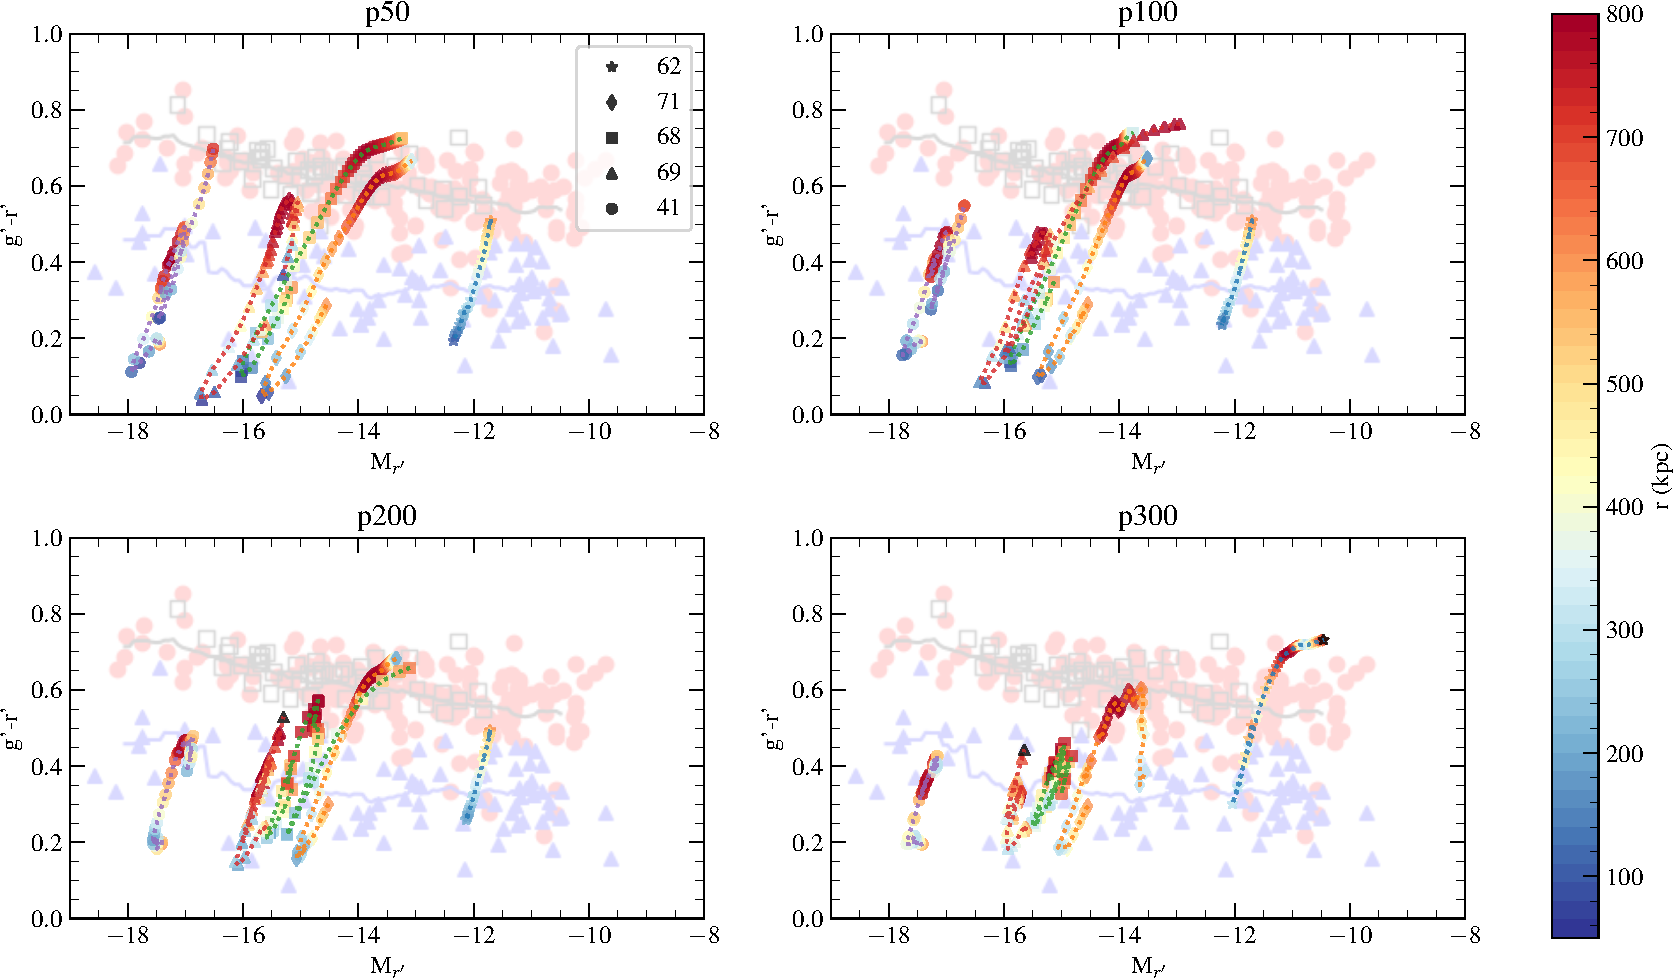
\includegraphics[width=\textwidth]{04.2_color_magnitude_Aku_g-r_rt_criterion_r.pdf}
\caption{SDSS bands colour magnitude diagram of galaxies on different orbits compared to Fornax dwarf catalogue of \citet{Venhola2019}.
% TODO ask permission for the overlay or use catalogue datapoints.
Red and blue colour for the data points in the background represent dwarf elliptical (dE) and late type galaxy respectively, classified by eye on the base of morphology.
Empty squares are nucleated dE.
Data tracks of simulated galaxies are shown overlaid colour coded by the clustercentric radius.
The tracks are limited to bound galaxies \ie{} they are drawn with snapshots for which condition \eqref{eq:tidal_radius_condition} holds.
}
\label{fig:g-r}
\end{sidewaysfigure}
\begin{sidewaysfigure}
\centering
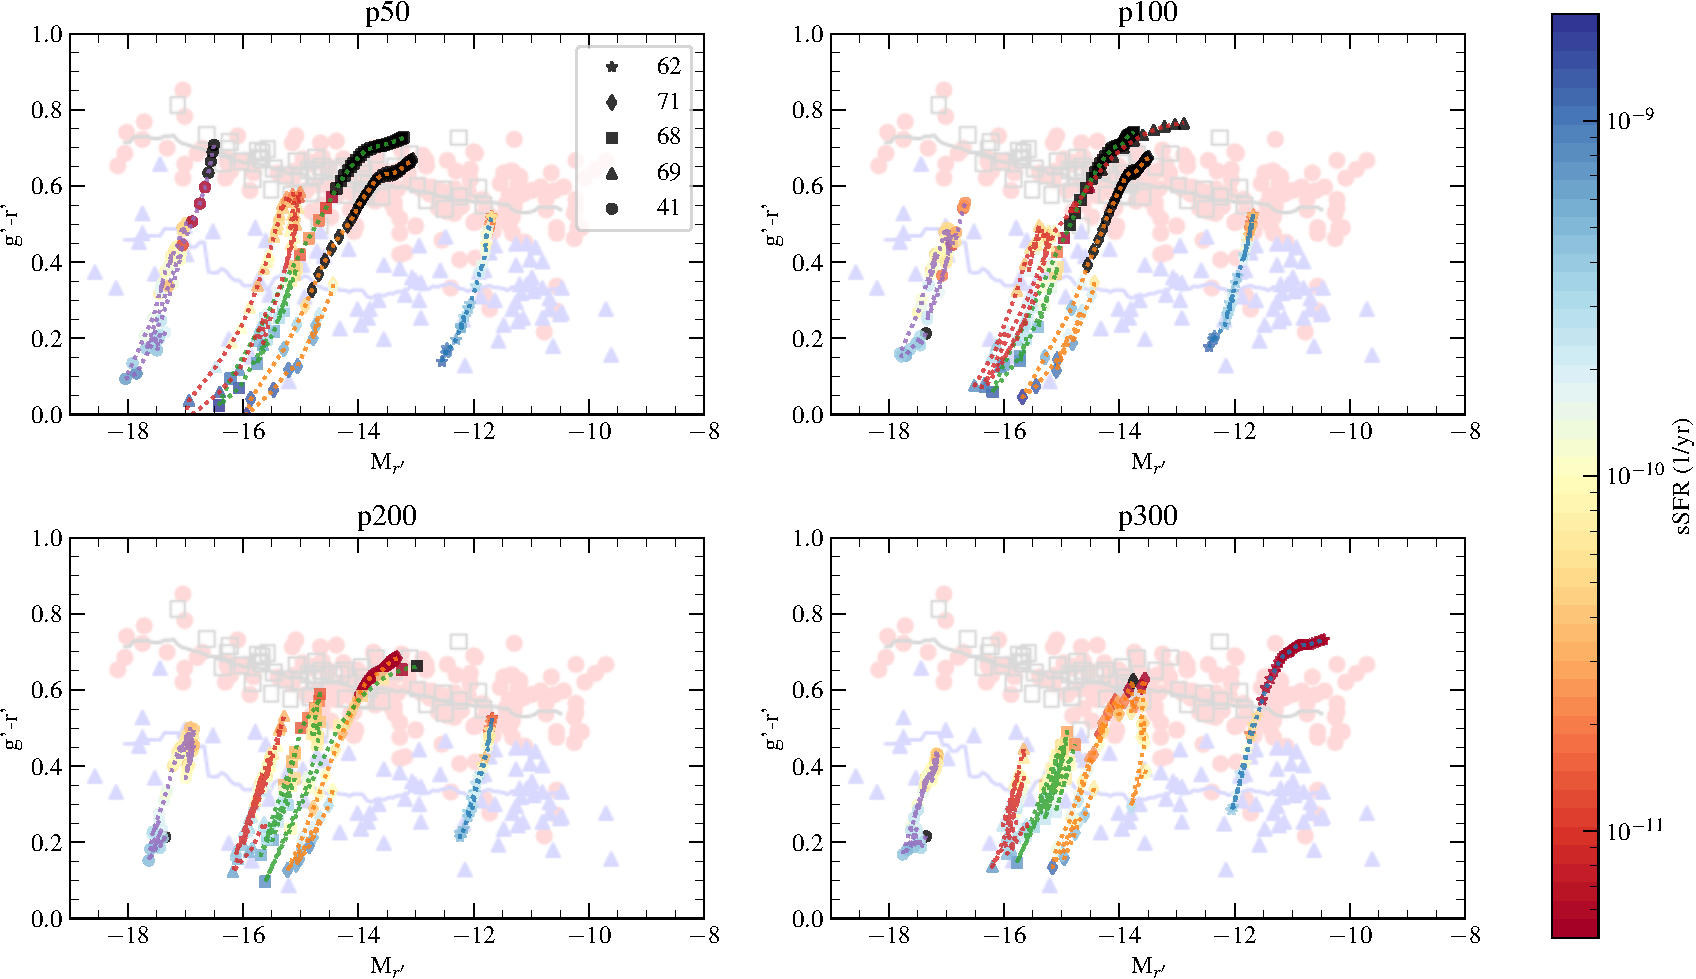
\includegraphics[width=\textwidth]{04.3_color_magnitude_Aku_g-r_rt_criterion_r_sfr.pdf}
\caption{Same as Figure~\ref{fig:g-r}, with point color coded with the specific star formation rate.
Black points are snapshots with no star formation.
}
\label{fig:g-r_sfr}
\end{sidewaysfigure}


\section{HI size mass relation during infall}
\begin{figure}[ht]
  \centering
  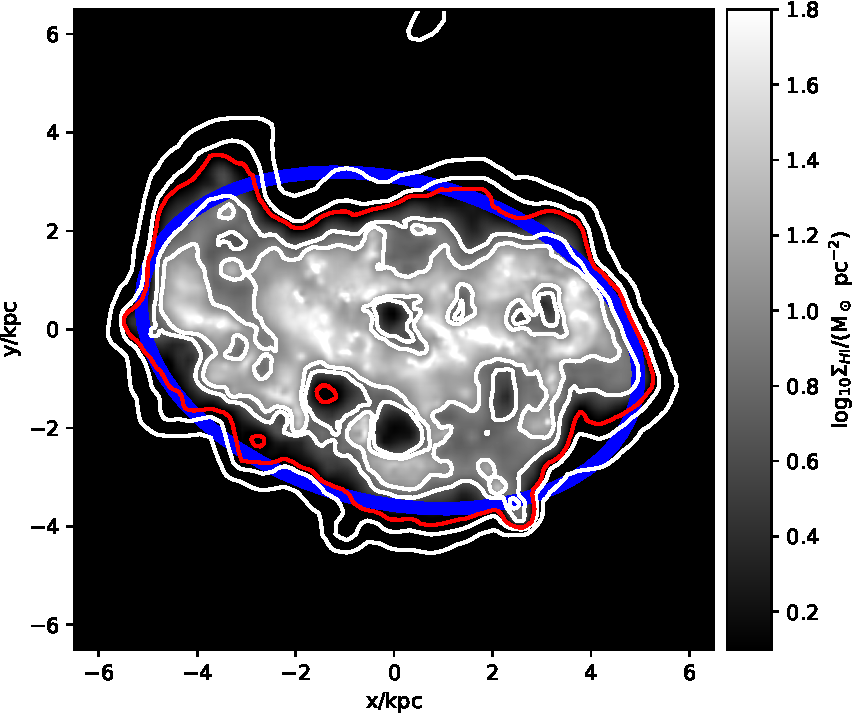
\includegraphics[width=0.83\textwidth]{hi_ell_69p200s11}
  \caption{\Hi{} map for a snapshot of simulation 69 at the beginning of the infall.
    In white the contours [$0.1, 0.5, 1, 5, 10$]~M$_\odot\,$~pc$^{-2}$ of the projected \Hi{} density $\Sigma_{\text{\Hi{}}}$.
    In blue the ellipse fit on the $1$~M$_\odot\,$~pc$^{-2}$ contour, shown in red.
  }
  \label{fig:hi_ellipse}
\end{figure}

\begin{figure}
  \centering
  \begin{subfigure}[t]{0.83\textwidth}
    \centering
    \caption{Simulation ID 71}
    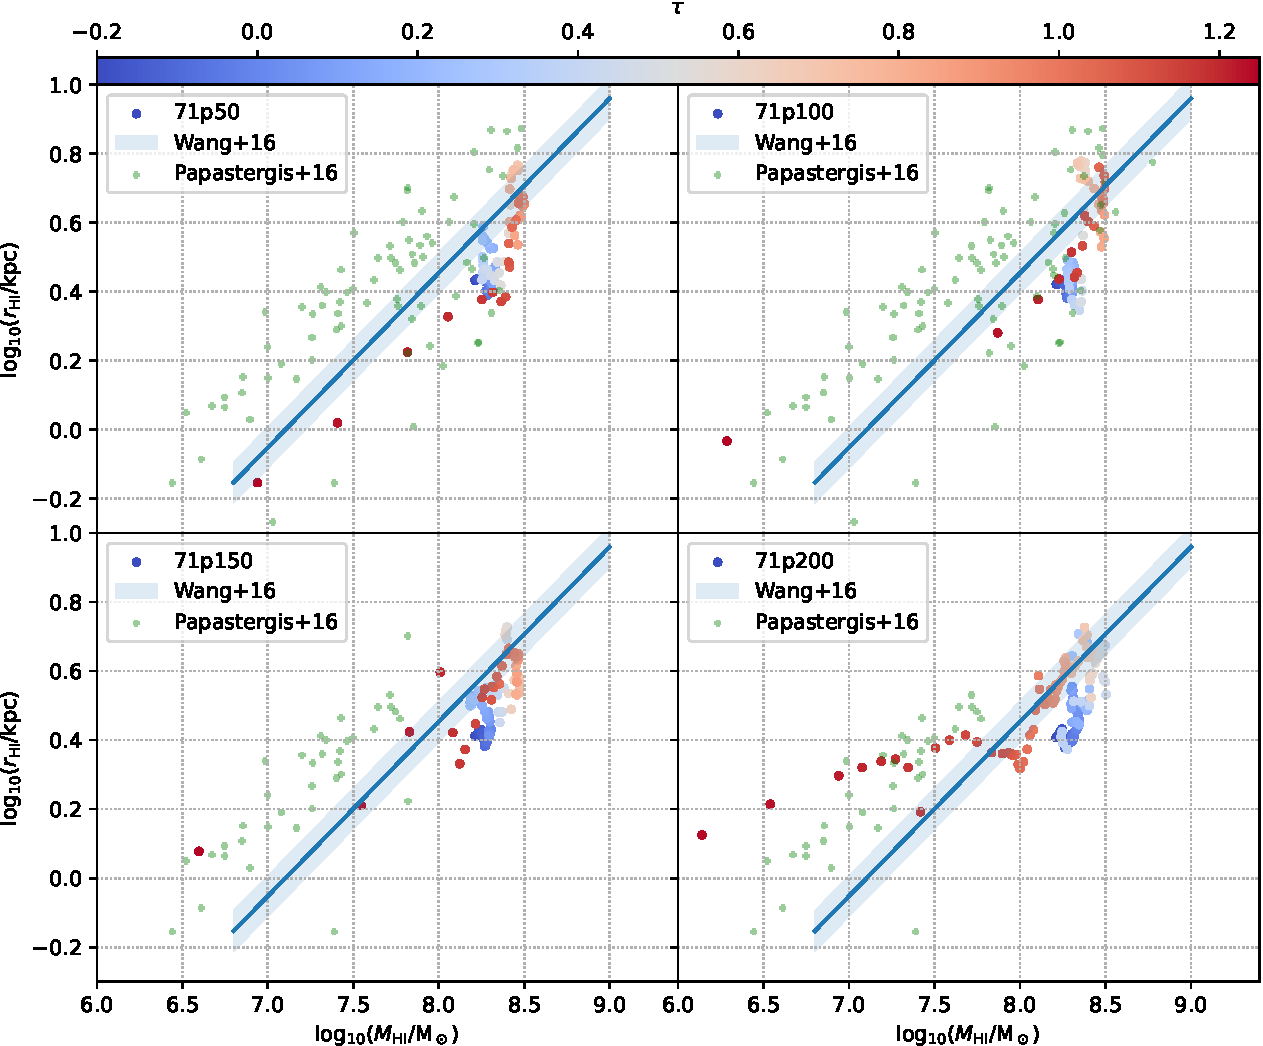
\includegraphics[width=\textwidth]{05_HI_analysis_multiorbit_71.pdf}
  \end{subfigure}\\%[1.5ex]
  \begin{subfigure}[t]{0.83\textwidth}
    \centering
    \caption{Simulation ID 69}
    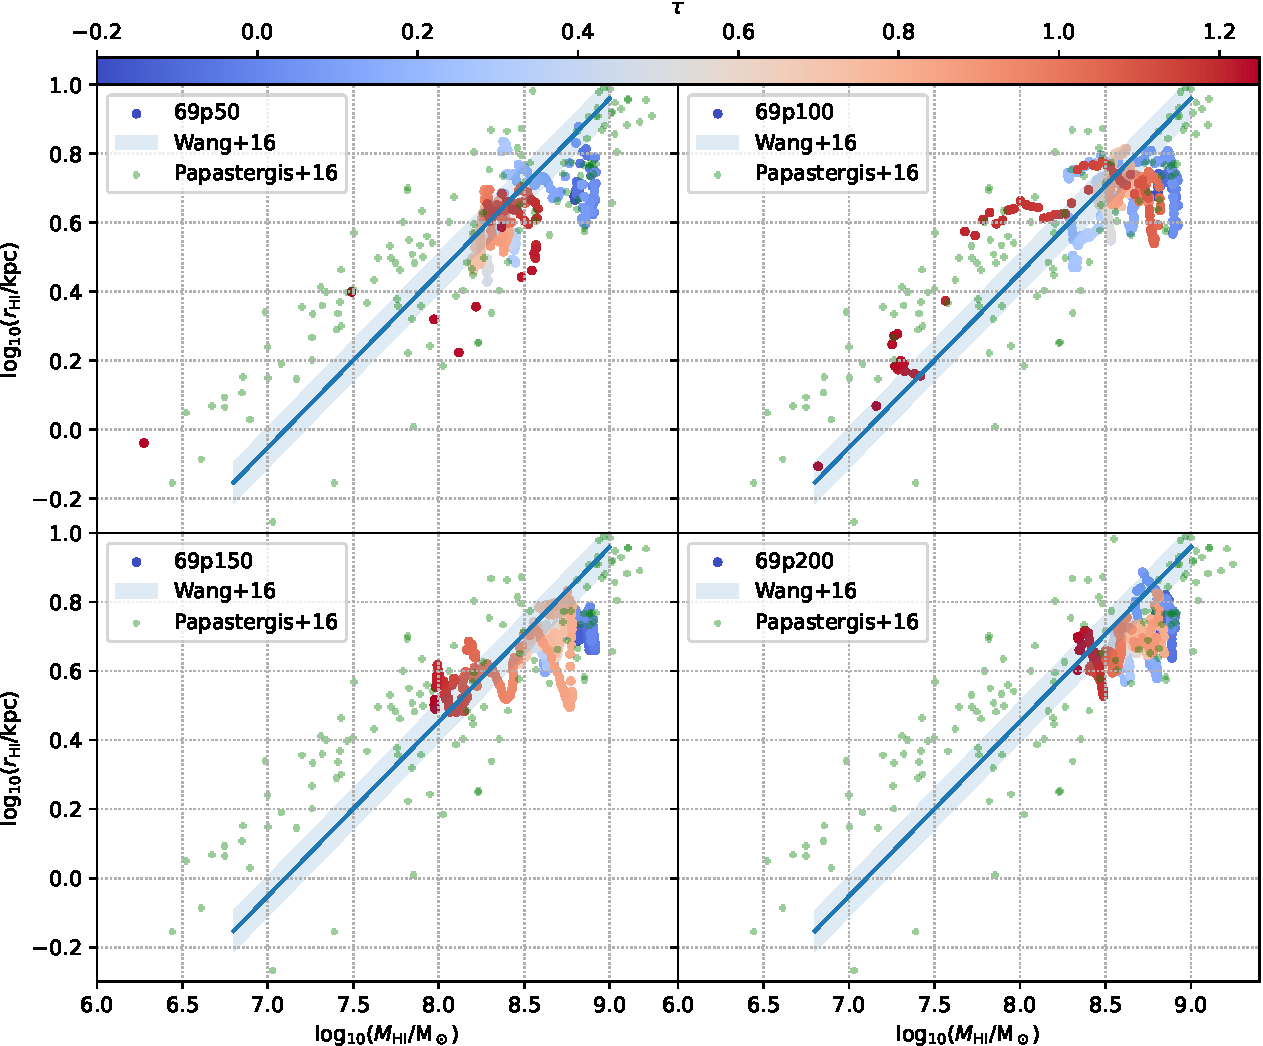
\includegraphics[width=\textwidth]{05_HI_analysis_multiorbit_69.pdf}
  \end{subfigure}
  \phantomcaption
  \label{fig:hi_size_mass}
\end{figure}
\begin{figure}[ht]
  \centering
  \ContinuedFloat % continue from previous page
  \begin{subfigure}{0.83\textwidth}
    \caption{Simulation ID 41}
    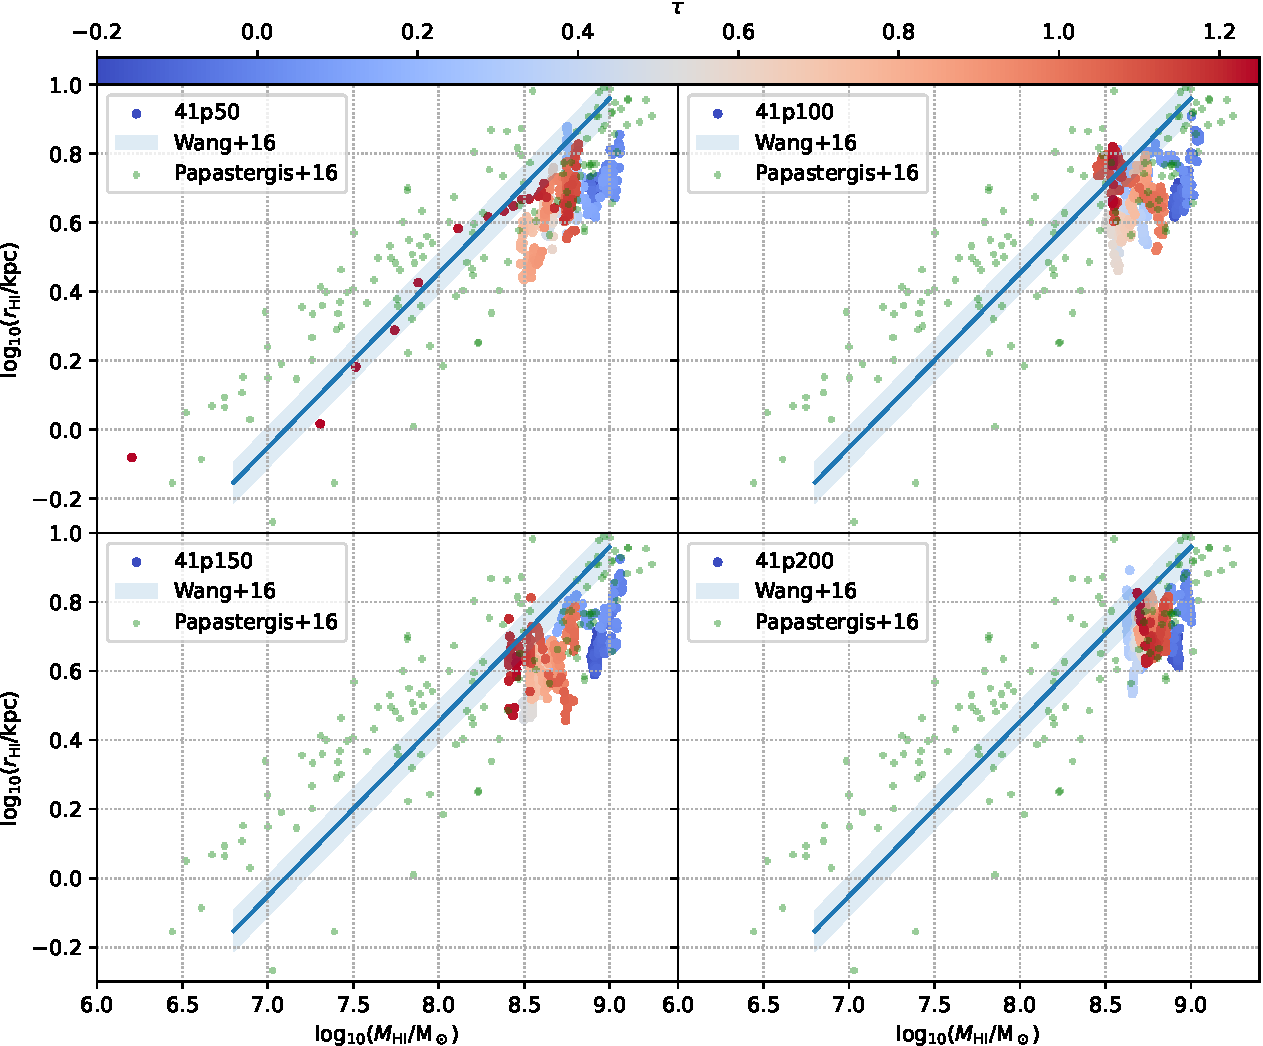
\includegraphics[width=\textwidth]{05_HI_analysis_multiorbit_41.pdf}
  \end{subfigure}
  \caption{\Hi{} size-mass relation for simulation ID 71, 69 and~41.
    The relation of \citet{Wang2016} and data of \citet{Papastergis2016} are shown.
    Each subpanel corresponds to a different pericenter distance.
    }
\end{figure}

\citet{Stevens2019} show how inevitable is the size-mass relation of neutral hydrogen, even during stripping phases.
Our simulations can be checked on the \Hi{} size-mass plane.
We post-processed our simulations to obtain the neutral hydrogen fraction, $\neutralfraction$, of each gas particle.
This is done leveraging the models explained in Section~\ref{sec:extended_gas_physics}.
In particular, the \Hi{} fraction of a gas particle is computed based on tabulated data from \citet{DeRijcke2013} as a function of density, temperature, composition, and redshift:
\[\neutralfraction = \neutralfraction(T, \feh, \mgfe, z, \rho),\]
resulting in a \Hi{} mass consistent with the sub-grid model employed during the simulations.
As in \citet{Verbeke2017}, we computed the \Hi{} mass by integrating the \Hi{} column density $\Sigma_{\text{\Hi}}$.
To compute the \Hi{} radius, we fit an ellipse to the $1$~\Msun{}~pc$^{-2}$ contour of the \Hi{} map (as shown in Figure~\ref{fig:hi_ellipse}) and $r_{\text{\Hi}}$ is thus defined as its major axis.


In Figure \ref{fig:hi_size_mass} we show the behaviour of the gas of three different simulations on four different orbits each.
The snapshots have been oriented following the assumption that the infinitely distant observer lies on the plane of the orbit of the galaxy.
We see that our dwarfs stay on the \Hi{} size-mass relation as computed by \citet{Wang2016}:
\begin{equation*}
  \log r_{\text{\Hi}} = (0.506 \pm 0.003) \log M_{\text{\Hi}} -(3.594 \pm 0.009).
\end{equation*}
The slope of $0.5$ implies that the \Hi{} mass is proportional to the surface area of the \Hi{} disk.
Also, data from the ALFALFA blind survey \citep{Papastergis2016} is used for comparison.
For the least massive galaxy (simulation ID 71) on the most radial orbits, the relation is followed closely.
In case of no stripping (high pericenter distances) the snapshots lay within the scatter of the data. On the other hand, when there is stripping (for the simulation ID~41, only for the orbit on $50$~kpc pericenter), the snapshots move along the relation on the mass-size plane.
In other words, the surface density of \Hi{} is constant not only among different galaxies but also over time when a galaxy undergoes stripping.

\section{Kinematics}
To correctly compute galaxy kinematics we have to take into account the rotation of the moving box.
The details on how to recover the correct kinematics in our setup are shown in \refsec{sec:correct_kinematics}.

\subsection{Comparison with simulated galaxies in the field}
We compare the specific stellar angular momentum $j_s$ of particles within a sphere of radius $10$~kpc from the center of the galaxy for both a simulation in the moving box as well as for a run in isolation.
We notice in Figure \ref{fig:j_s_moria} an increase of $j_s$ in correspondence to pericenter passages.

The combination of high-velocity newly born stars and the gravitational energy injection given by the cluster at pericenter, result in a spin-up of the galaxy with respect to its evolution in the field.
% TODO metallicity gradient?

\begin{figure}
\centering
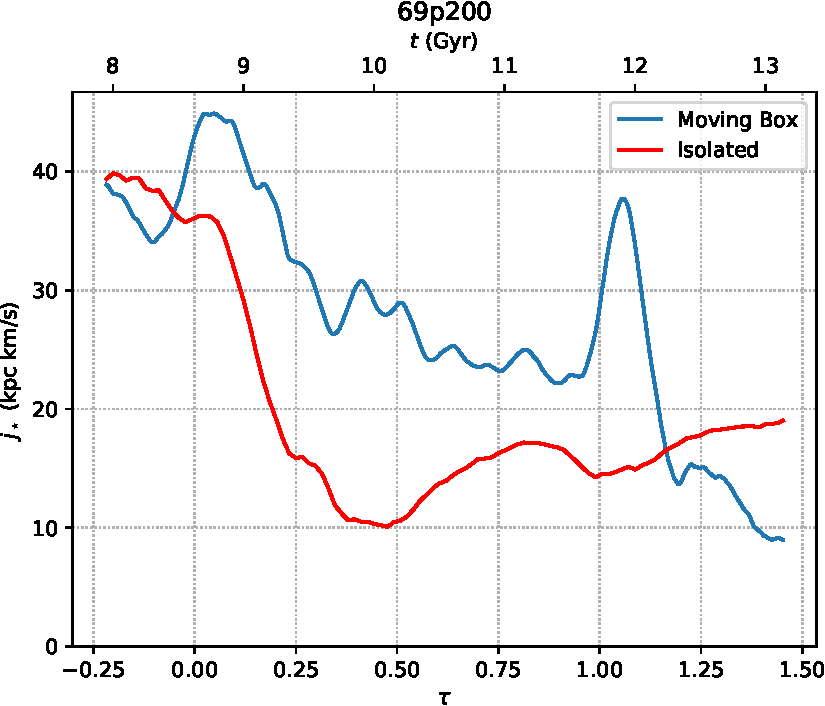
\includegraphics[width=0.8\textwidth]{15.0_angmom_inertial_moria.pdf}
\caption{Comparison between the norm of the specific angular momentum $j_s$ for the simulation ID 69 on a 200 kpc orbit and the correspondent isolated MoRIA run.}
\label{fig:j_s_moria}
\end{figure}

\subsection{Angular momentum and specific angular momentum proxy $\lambda_R$}
We compute the specific stellar angular momentum proxy $\lambda_R$ starting from SPH luminosity-weighted velocity and velocity dispersion maps as defined in \citet{Emsellem2007}: %\citet{Toloba2015}
\begin{equation}
 \lambda_R = \dfrac{\sum_i F_i R_i |V_i|}{\sum_i F_i R_i \sqrt{V_i^2 + \sigma_i^2}}
 \label{eq:lambda_r}
\end{equation}
with $i$ the pixel index, $F_i$ its flux, $R_i$ the distance of the pixel from the galaxy center, with $V_i$ the mean line-of-sight velocity of a pixel and $\sigma_i$ its velocity dispersion.
This parameter has been introduced to better capture the spatial information included in the kinematic maps.
As opposed to the classical $v/\sigma$ indicator, $\lambda_R$ has been designed to distinguish between galaxies with kinematically decoupled components (KDC),
which in some cases exhibit large $v/\sigma$ typical of rotation-supported galaxies, despite their rotation being confined to the central regions.

An example of the maps from which $\lambda_R$ is computed for our simulation setup are shown in Figure~\ref{fig:maps_lambda_r}.
The $V_{LOS}$ and $\sigma$ map are computed with SPH interpolation, using the luminosity in $\mathrm{V}$-band to weight the contribution of particles along the line of sight.
Some authors \citep[e.g.][]{Schulze2018,Pillepich2019} use non-weighted quantities taken directly from the particles to compare simulations and observations. %, even if what is observed are luminosity-weighted measures.
This approach makes the comparison with observations more difficult since all the information that we get is luminosity weighted \citep{Walo-Martin2020}.

\begin{figure}[t]
\centering
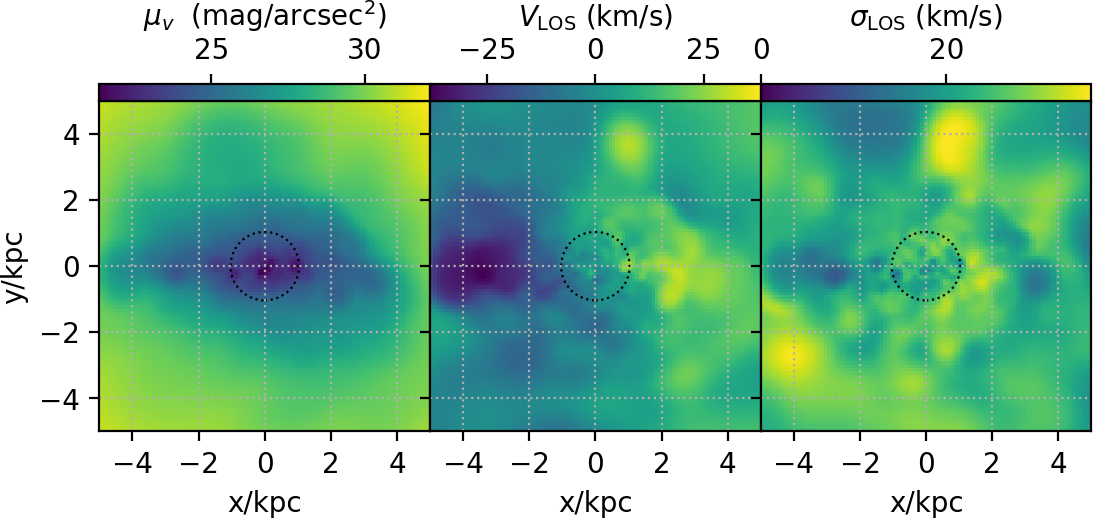
\includegraphics[width=\textwidth]{mu_v_sigma_69p200s60_sideon.png}
\caption{$\mu_\mathrm{v}$ surface brightness map and SPH v-band luminosity weighted maps of line of sight velocity and velocity dispersion $\sigma$ for a snapshot of the simulation ID 69 around first pericenter passage.
The galaxy is projected edge-on, with the angular momentum vector lying on the $xy$ plane.
A dotted circle of radius $R_e$ is shown.}
\label{fig:maps_lambda_r}
\end{figure}
\begin{figure}[t]
  \centering
  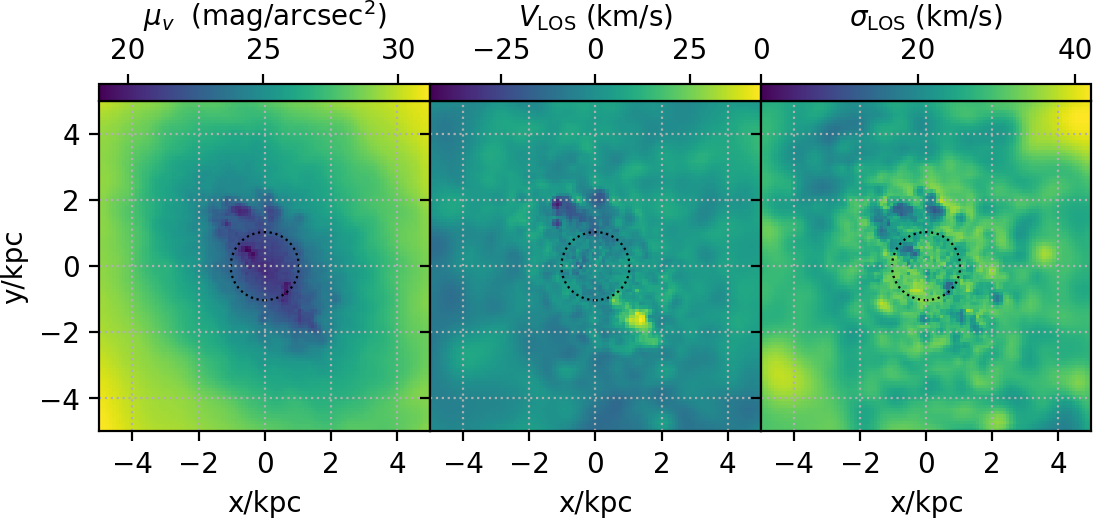
\includegraphics[width=\textwidth]{mu_v_sigma_41p200s60_sideon.png}
  \caption{Same as Figure~\ref{fig:maps_lambda_r} for simulation ID 41. Note the peak in $V_{\mathrm{LOS}}$ outside of $R_e$.}
  \label{fig:maps_lambda_r_41}
\end{figure}

\begin{figure}[h!]
\centering
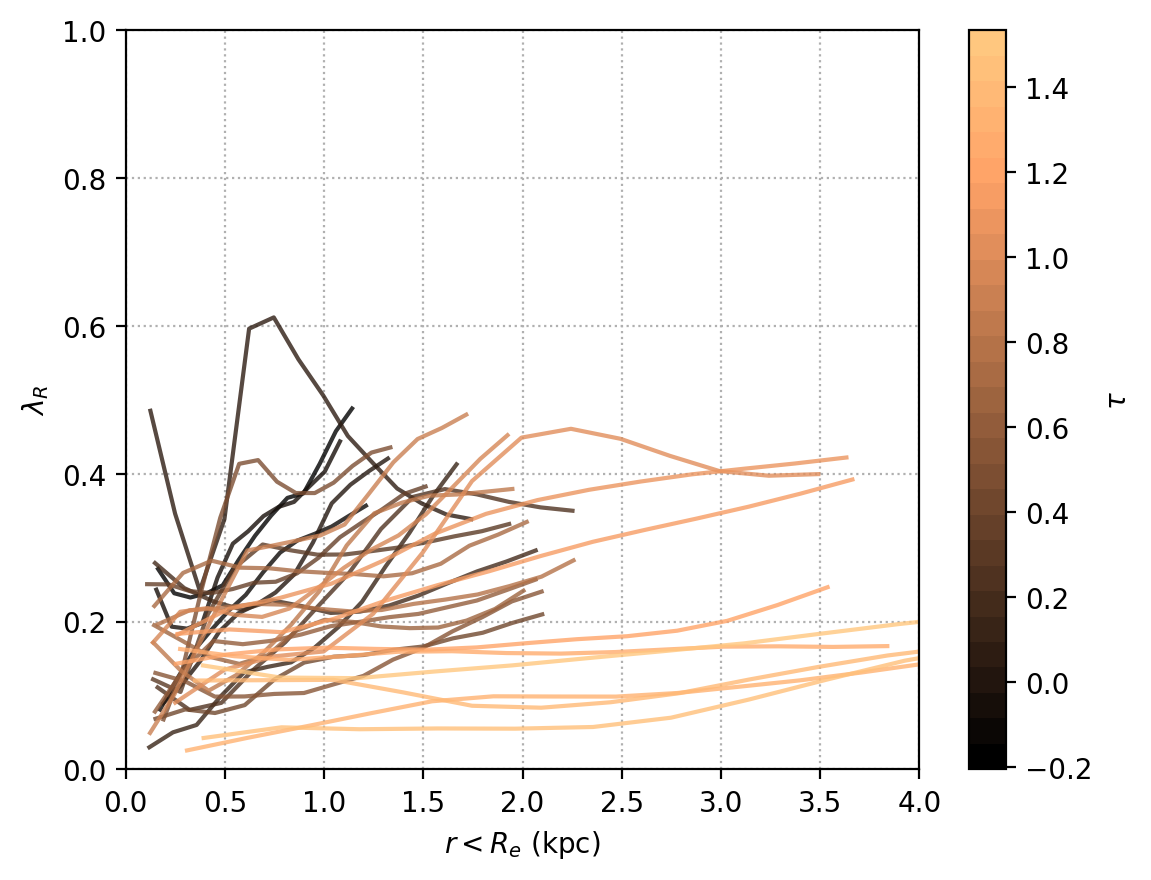
\includegraphics[width=0.8\textwidth]{lambda_r_profile_69p100_each20_up_to_r_e_15bin}
\caption{$\lambda_R$ profiles for ID 69 on a 100 kpc orbit color coded with time normalized by radial period.
The $\lambda_R$ profile is shown up to the corresponding $R_e$.}
\label{fig:lambda_r_profile}
\end{figure}

It is possible to compute the radial profile of $\lambda_R(r)$ including in the summation of eq. \eqref{eq:lambda_r} only those pixels that have a galactocentric distance smaller than $r$.
The profile itself and the value $\lambda_R(R_e) = \lambda_{R_e}$ is used to distinguish between fast and slow rotators.
\citet{Emsellem2007} defines galaxies with $\lambda_{R_e} < 0.1$ as ``slow rotators'' and those with $\lambda_{R_e}>0.1$ as ``fast rotators''. While falling into the cluster, galaxies evolve from being classified as having a fast-rotator profile to slow rotator \citep[\cf{} also][]{Emsellem2011}.
We show an example of the profile in Figure~\ref{fig:lambda_r_profile}, for simulation ID 69 as a function of time.
It is clear that, in a time-frame that is short compared to the lifetime of the galaxy, $\lambda_R$ undergoes significant changes, both locally, as a function of radius, and averaged over the whole galaxy.
In particular, the changes are large enough to cause the galaxy to cross the slow/fast rotator classification threshold.
Also, it is worthwhile to note that the value of $r$ adopted affects whether a galaxy is classified or not as a slow rotator.

There is a complex interplay between $R_e$, $\sigma$ and the rotational velocity while the galaxy is on its orbit.
$R_e$ increases with time whereas velocity dispersion and the rotation velocity at a fixed radius tends to decline.
No single phenomenon can be called to explain the $\lambda_R$ profile behaviour.
The result of this joint evolution is $\lambda_{R_e}$ decreasing with time.

% Obviously this distinction depends on the real inclination of the galaxy, as it appears in the sky. % TODO possible to include inclination in a plot?

It has been shown in the \textsc{SMAKCED} survey of 39 early-type galaxies in the Virgo cluster \citep{Toloba2014, Toloba2015} that the so classified fast-rotator galaxies in the outer region of the cluster rotate faster than the fast rotators in the center of the cluster.
Therefore, in this case, observed specific angular momentum $\lambda_R$ is correlated with cluster-centric distance. % FIXME \citep{Bidaran2020}. citep DEugenio2015
It is indeed hypothesized, that after pericenter passages and a long time in the cluster, galaxies are heated up and transformed into slow rotating dEs.
This scenario is confirmed by our simulations where dwarf irregulars are converted into early-type galaxies, and with time their kinematics is transformed into the one of slow rotators.

In our case, however, the correlation of $\lambda_R$ with clustercentric distance is mild and affected by the very noisy and time-dependent nature of the angular momentum proxy.
For example in simulation ID 69, as shown in Figure~\ref{fig:lambda_r_j_s}, $\lambda_R$ behaviour is very oscillatory %and quite prone to bursty star formation which can abruptly affect its value.
%In our measurements, $\lambda_R$
and fails to distinguish pericenter passages unequivocally.

\begin{figure}
  \centering
  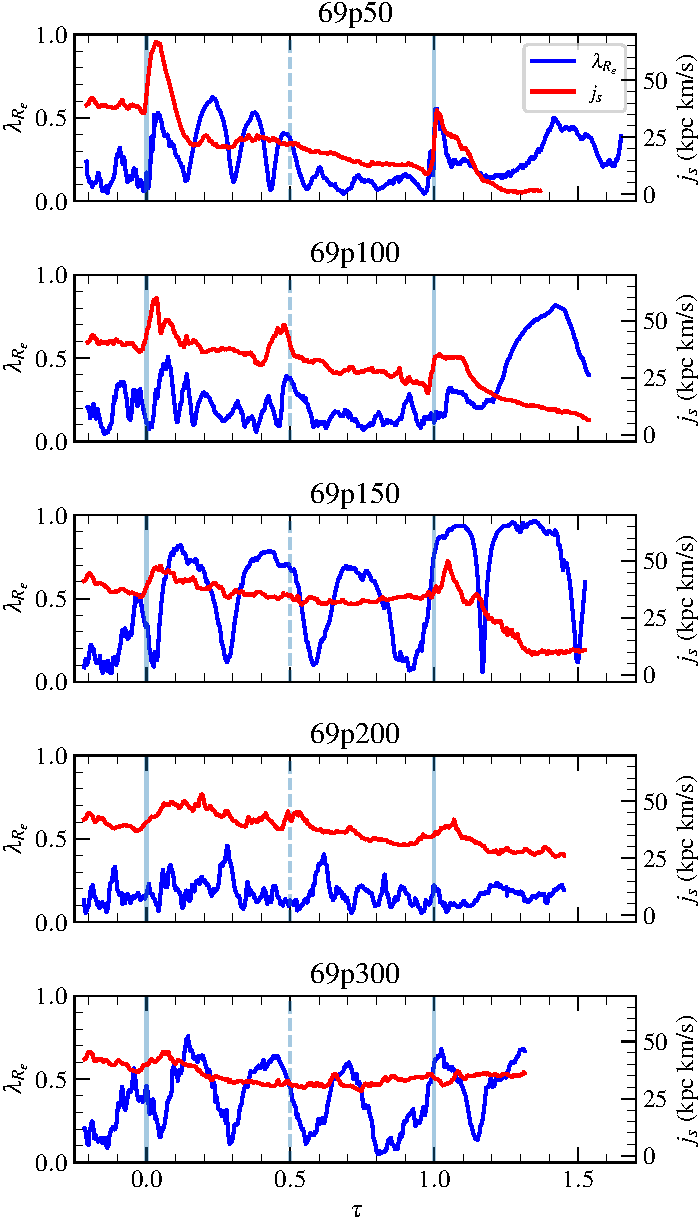
\includegraphics[height=0.9\textheight]{02.2_lambda_re_vs_js}
  \caption{Stellar specific angular momentum proxy $\lambda_R$ and specific angular momentum of star particles $j_s$ for the simulation ID 69 on multiple orbits. The measurements have been taken by observing the galaxy from the plane of the orbit, recreating the condition of a fixed observer.
  Note the relatively stable values of $j_s$ (a conserved quantity) compared to the oscillatory nature of $\lambda_R$, which oscillates by more than $50$\%.}
  \label{fig:lambda_r_j_s}
\end{figure}

\subsection{Relation between $\lambda_R$ and physical angular momentum}
In Figure~\ref{fig:lambda_r_j_s}, in order to compare $\lambda_R$ and the angular momentum of the galaxies in an observationally motivated way, we chose to observe the galaxy from the plane of the orbit, not changing its point of view along its evolution.
Given the spin of the galaxy in correspondence of the pericenter (as shown in the previous section), from this point of view the pericenter passage should be visible in $\lambda_R$ at the highest extent.
In Figure~\ref{fig:lambda_r_j_s}, $j_s$ is the norm of the specific angular momentum vector and it is in fact affected by pericenter passages for radial orbits, whereas it is relatively conserved for more circular orbits.

It is striking how $\lambda_R$ oscillates along the orbit (\eg{} see panel $69$p$150$) and this highlights how inherently variable $\lambda_R$ is.
It is thus clear that - at least for the class of galaxies we consider - the snapshots in Figure~\ref{fig:lambda_r_profile} are not representative of the mean value of $\lambda_R$,
and an instantaneous measurement of $\lambda_R$ cannot be used to classify a galaxy as slow/fast, because of the large time-dependent variation.

% \begin{equation}
% \vect{j}_s = \sum_{i\in S} \vect{r}_i\cross\vect{v}_i,\quad \text{where } S\equiv\{k: \norm{\vect{r}_k} < 10 \text{~kpc.}\}
% \end{equation}
% ($\vect{j}_s = \vect{J}_s/M_\star$ where $J_s$ is the total angular momentum and $M_\star$ the stellar mass of the galaxy)
% We compare $\vect{j}_{s}$ with $\lambda_R$ in Figure \ref{fig:lambda_r_j_s}.


%We would like to investigate more the oscillating behaviour $\lambda_R$ shown in Figure~\ref{fig:lambda_r_j_s}.
\citet{Emsellem2007} in their Appendix A, present a description of three main effects at play when trying to recover the apparent angular momentum: projection effects, luminous distribution and mass distribution of the galaxy.
In their formal exposition, they describe the approximations made to relate $\lambda_R$ (which is obtained from the properties of the galaxy measured from the point of view of the observer) to the intrinsic spin parameter~$\lambda$ \citep[p. 757]{BinneyTremaine2008}:
\begin{equation}
  \lambda = \frac{J\sqrt{|E|}}{G M^{2.5}} = \frac{j\sqrt{|E|/M}}{G M},
  \label{eq:spin_coefficient}
\end{equation}
where $J = jM$ is the total angular momentum, $M$ the galaxy of the mass and $E = T + W$ the total energy of the system, where
$T= 1/2\, M\, V^2_\mathrm{rms}$ and $W = -GM^2/r_g$ the kinetic and potential energy, respectively, which are linked by the scalar virial relation $T = -\frac 1 2 W$.

The approximations of using the projected radius $R$ instead of both the gravitational radius $r_g$ and the distance from the spinning axis $r$, are taken into account through the coefficients $\kappa_R$ and $\kappa_J$;
similarly, using the second order velocity moment $V^2+\sigma^2$ instead of the mean-square speed of the system $V^2_{\mathrm{rms}}$, is considered through the coefficients $(\kappa_V, \kappa_\sigma)$.
All in all these four coefficients grasp the effects of projection and of the luminous and mass distribution:
\begin{equation}
  \left\{
  \begin{array}{cl}
    j &= \kappa_J \langle R|V| \rangle, \\ [1ex]
    2E/M = V^2_{\mathrm{rms}} &= -\langle \kappa_V V^2 + \kappa_\sigma \sigma^2 \rangle, \\ [1ex]
    GM &= \kappa_R \left\langle R\left( \kappa_V V^2 + \kappa_\sigma \sigma^2 \right) \right\rangle. \\
  \end{array}
  \right.
  \label{eq:spin_vs_lambda_R}
\end{equation}
In the case of $\lambda_R$ the coefficients are set to: $\kappa_J/\kappa_R=\sqrt{2}$, $\kappa_V=\kappa_\sigma=1$.

\subsubsection{Comparing $\lambda_R$ with observables}

Given the possible interest observers may have in how much $\lambda_R$ is a tracer of the apparent angular momentum, we investigated the relation between the two in our simulations setup \citep[\cf{} the work of][]{Walo-Martin2020}.
We tried to use $\lambda_{R_e}$ as a starting point to compute the physical angular momentum.
To do so, we try to retrieve an approximate formula for the specific angular momentum which relies on observable quantities:
\begin{equation}
 j_s^* = \lambda_{R_e}\, R_e\, \sigma_e
 \label{eq:js*}
\end{equation}
where $\sigma_e$ is the line-of-sight velocity dispersion of star particles measured within an aperture of $R_e$.
For a fair comparison we compute the specific angular momentum $\vect{j}_{se}$ of star particles within $R_e$ (the projected effective radius).
\begin{equation}
  \vect{j}_{se} = \sum_{i\in S} \vect{r}_i\cross\vect{v}_i,\quad \text{where } S\equiv\{i: \norm{\vect{r}_i} < R_e.\}
\end{equation}
% This formula reasonably reintroduces physical dependency.
The relation between $j_{se} = \norm{\vect{j}_{se}}$ and $j_s^*$ is shown in Figure~\ref{fig:lambda_r_j_s_sigma}.
To simplify the treatment, as a first approximation, the snapshots have been rotated edge-on.

\begin{figure}
  \centering
  \begin{subfigure}[t]{0.93\textwidth}
  \centering
  \caption{ID 69}
  \label{fig:lambda_r_j_s_sigma_69}
  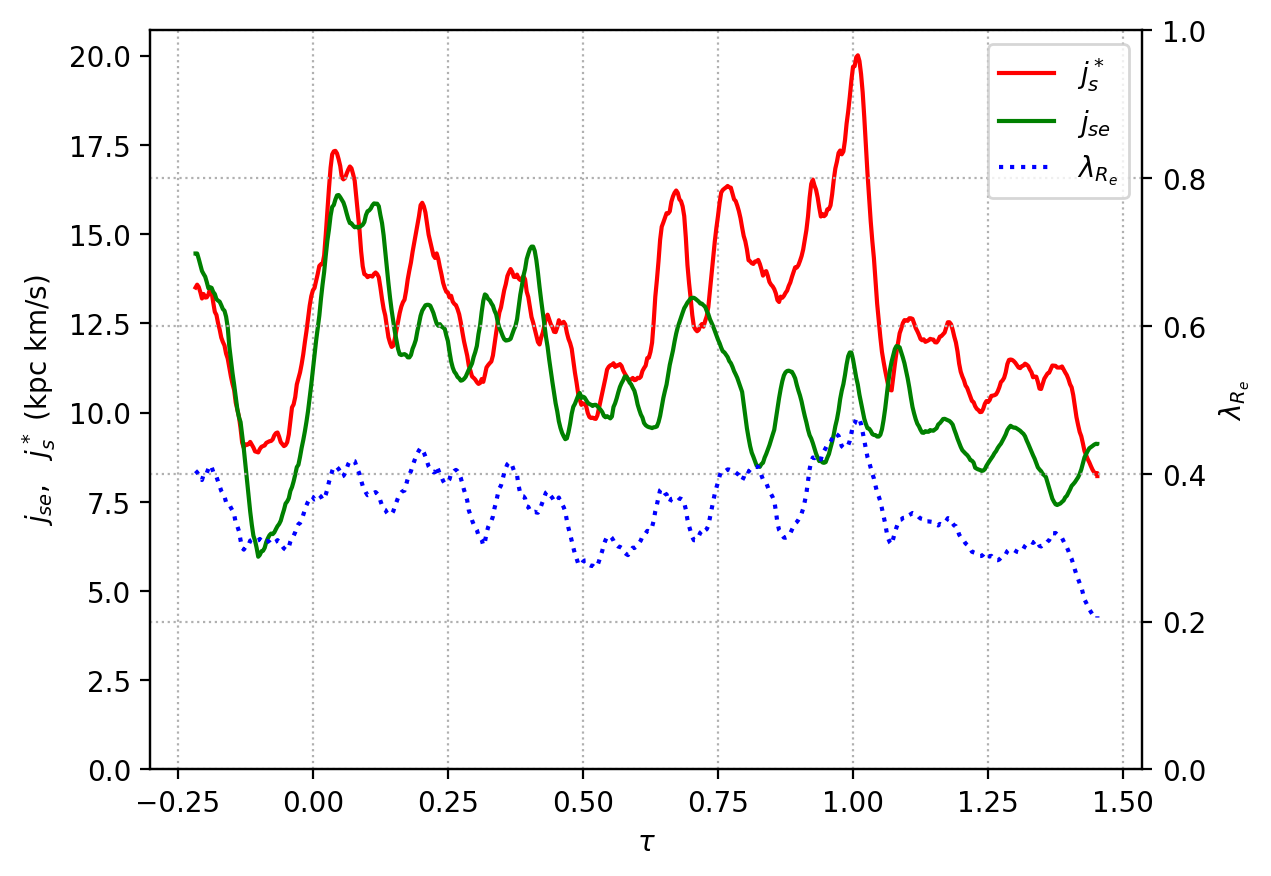
\includegraphics[width=\textwidth]{lambda_r_j_s_69p200r100}
 \end{subfigure}\\
 \begin{subfigure}[t]{0.93\textwidth}
  \centering
  \caption{ID 41}
  \label{fig:lambda_r_j_s_sigma_41}
  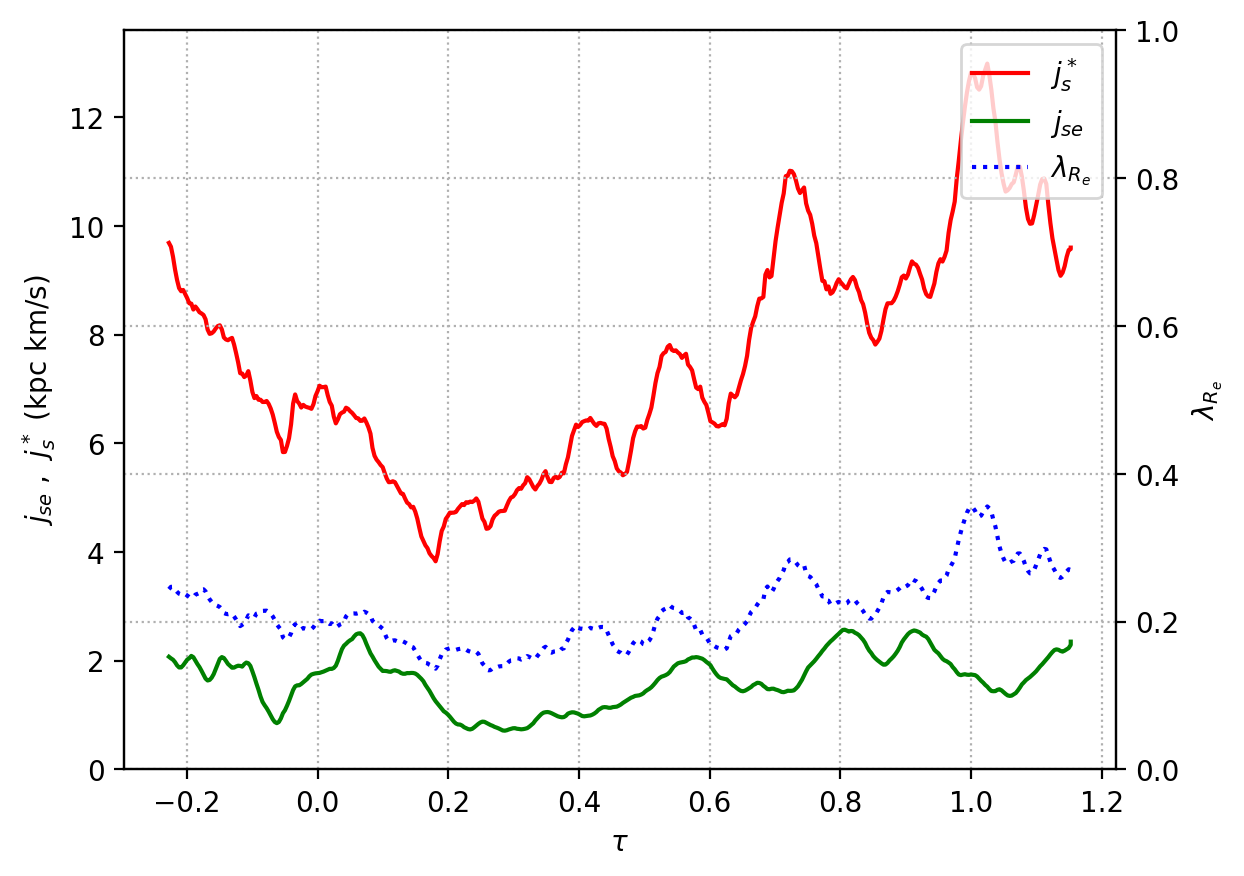
\includegraphics[width=\textwidth]{lambda_r_j_s_41p200r100}
 \end{subfigure}
%  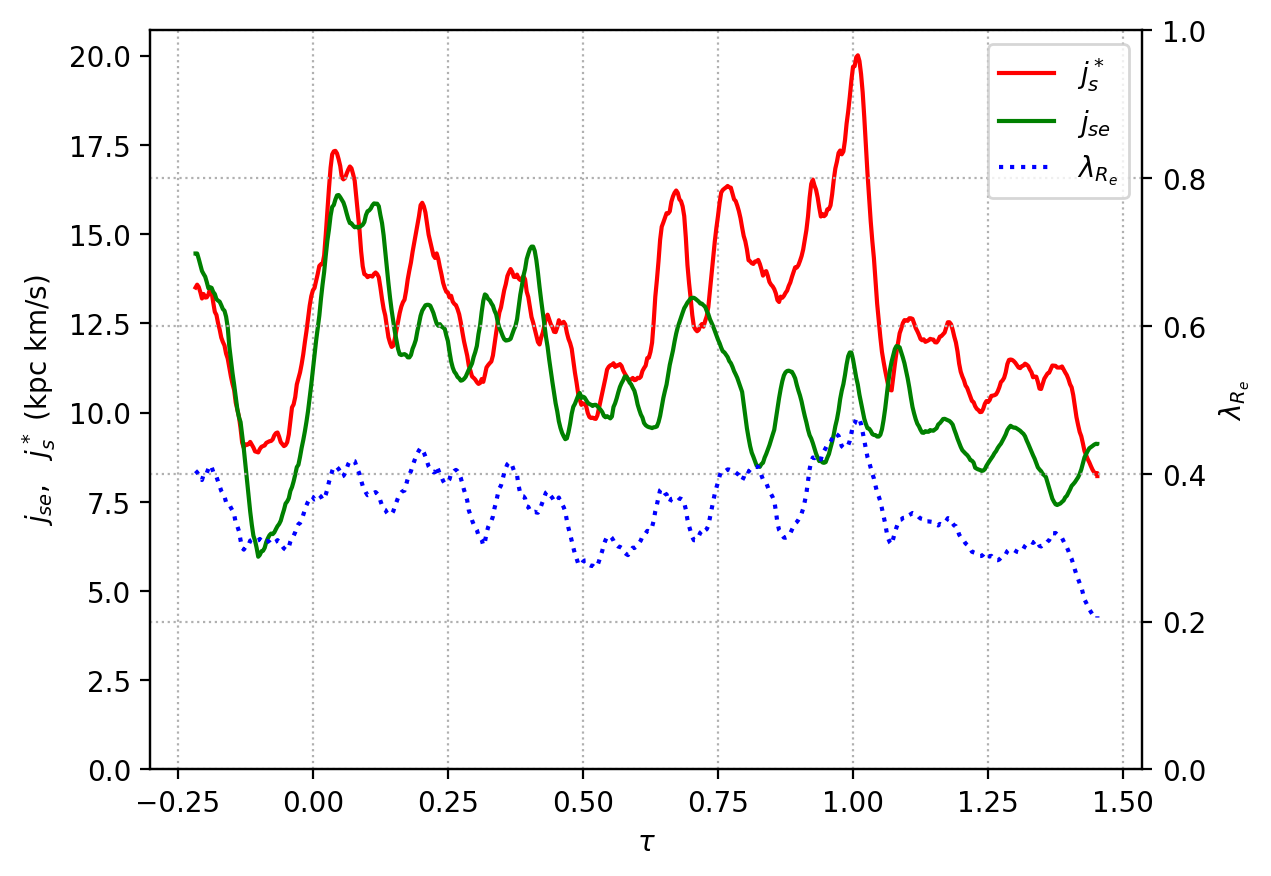
\includegraphics[height=0.42\textheight]{lambda_r_j_s_69p200r100.png}
  \caption{Comparison between specific angular momentum $j_{se}$ and $\lambda_{R_e}$ at the effective radius for simulation ID 69 and ID 41 on a 200~kpc orbit.
  $\lambda_{R_e}$ is computed viewing the galaxy side-on.
  Curves are smoothed using a rolling average of 0.2~Gyr.}
  \label{fig:lambda_r_j_s_sigma}
\end{figure}

It is interesting to see how for the case of simulation ID 69 in Figure~\ref{fig:lambda_r_j_s_sigma_69} the order of magnitude of $j_s^*$ is strikingly in accord with the measured $j_{se}$ from the particles.
In contrast, for simulation ID 41, there is no correlation.
Given that ID 41 shows an unusual velocity profile (the peaks of the line-of-sight velocity lay outside of $R_e$, as shown in Figure~\ref{fig:maps_lambda_r_41} we hypothesize that the limited radius used to compute $\lambda_{R_e}$ may cause the discrepancy.
Accordingly, we inspected the possibility that by computing both $j_{se}$ and $j_s^*$ within $2 R_e$ a tighter relation between them would emerge.
Figure~\ref{fig:lambda_2r_j_s_sigma} does not support this theory, and the gap between $j_{se}$ and $j_s^*$ increases for the doubled radial limit.

We conclude that in the dwarf-irregular regime covered by our simulations the adapted proxy $j_s^*$ computed in equation \eqref{eq:js*} is not a good tracker of angular momentum.


%As also found by, ... we confirm that it is very sensitive to recent episode of star formation, especially the ones due to gas stripping, where young stars are
% For these reasons in the case of dwarf irregulars it is not a good indicator of the real rotation of the galaxy.

\begin{figure}
  \centering
  \begin{subfigure}[t]{\textwidth}
    \centering
    \caption{ID 69}
    \label{fig:lambda_2r_j_s_sigma_69}
    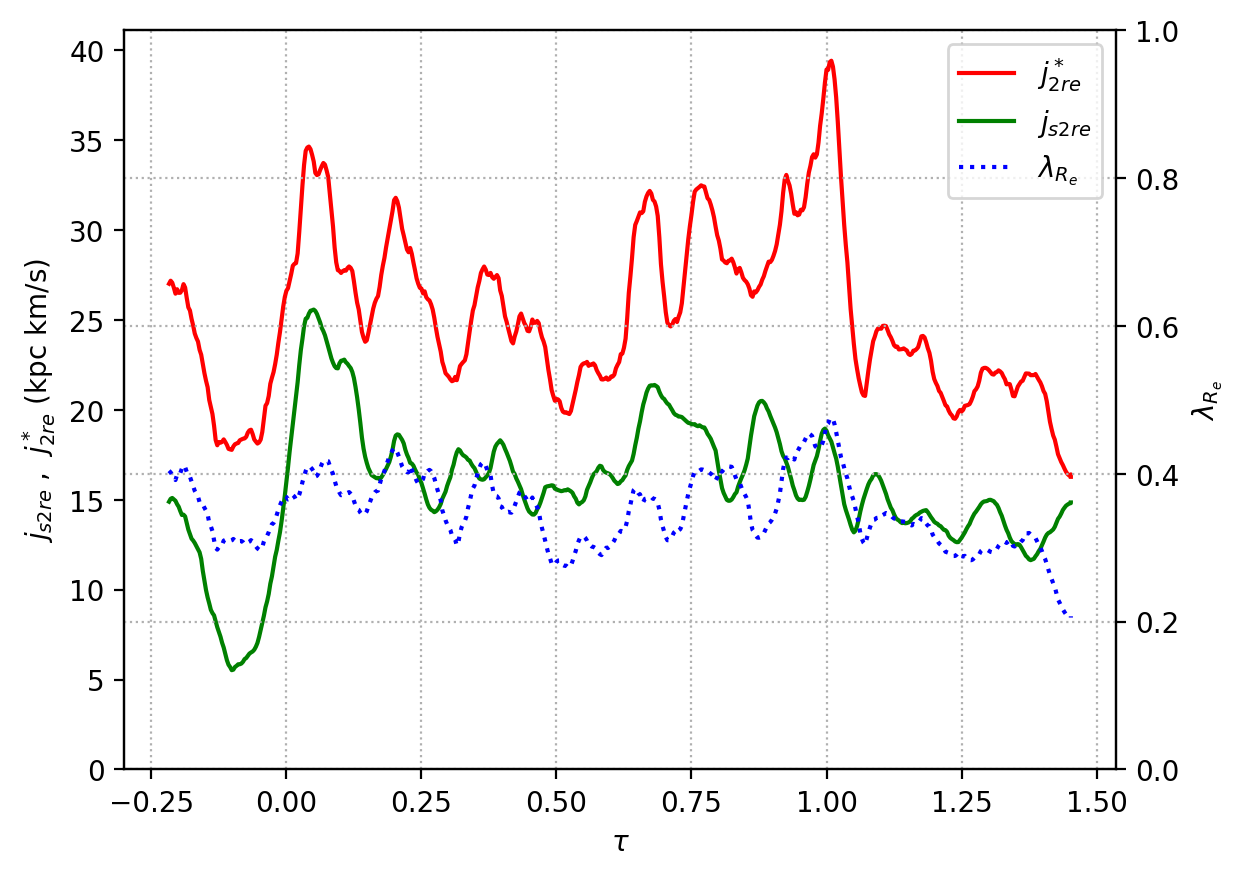
\includegraphics[width=0.93\textwidth]{lambda_r_j_s_69p200r100_2re_only}
  \end{subfigure}\\
  \begin{subfigure}[t]{\textwidth}
    \centering
    \caption{ID 41}
    \label{fig:lambda_2r_j_s_sigma_41}
    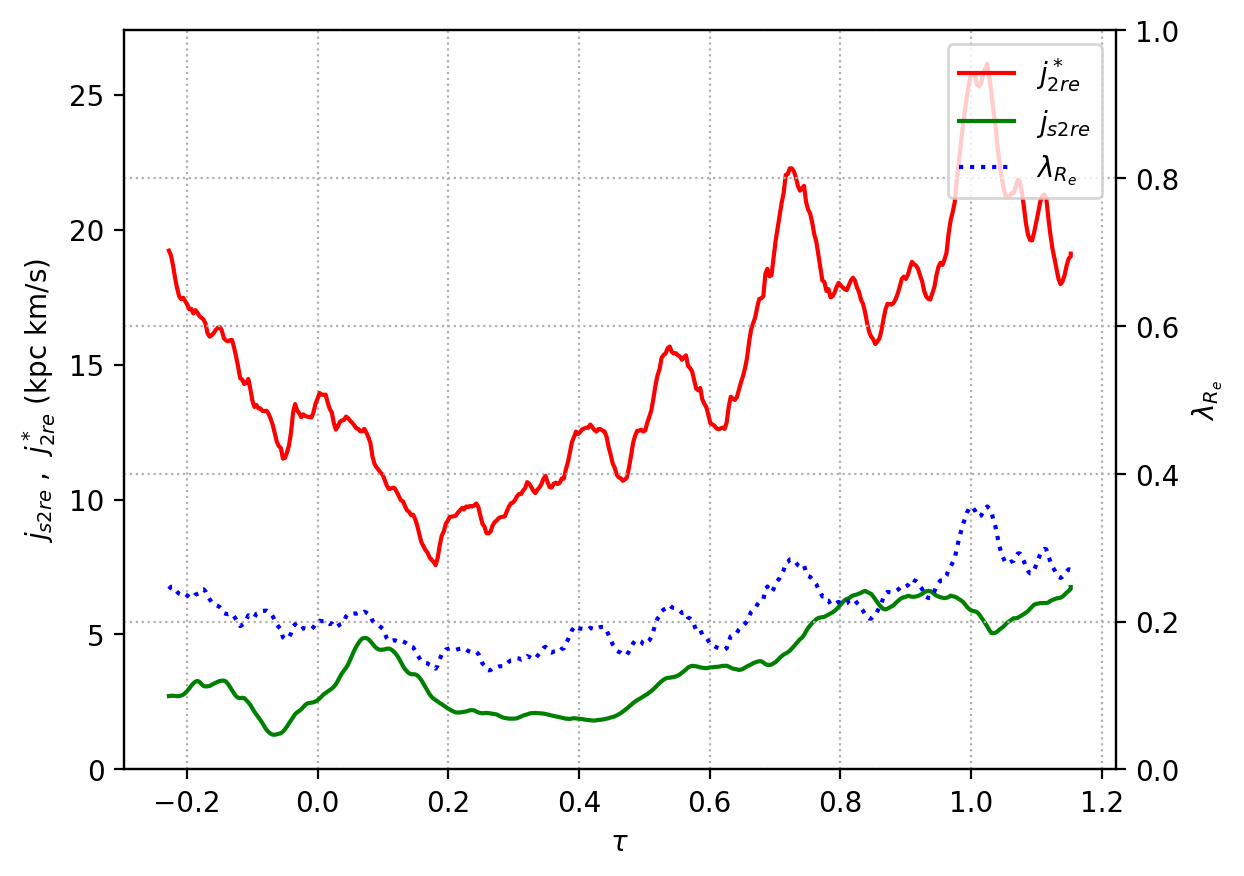
\includegraphics[width=0.93\textwidth]{lambda_r_j_s_41p200r100_2re_only}
  \end{subfigure}
  %  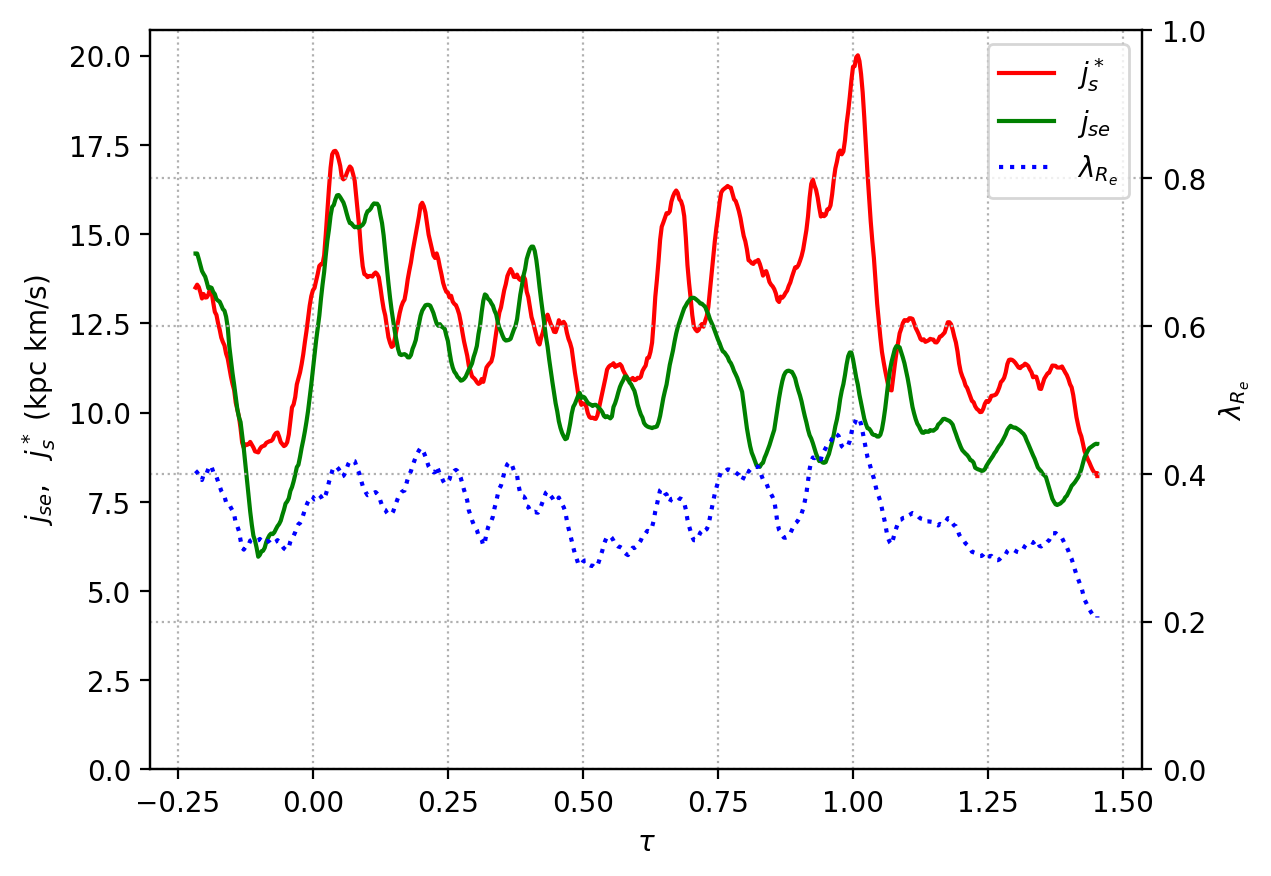
\includegraphics[height=0.42\textheight]{lambda_r_j_s_69p200r100.png}
  \caption{Same as Figure~\ref{fig:lambda_r_j_s_sigma}, but using the limit of $2 R_e$ to compute $j_{se}$ and $\lambda_R$.}
  \label{fig:lambda_2r_j_s_sigma}
\end{figure}

%\section{Conclusions}
%
%\begin{itemize}
% \item $\lambda_R$ is very variable with time in the dwarf irregular regime.
% \item It is sensitive to many things. % FIXME
% \item There can be cases in which depending on the projection and the size of the galaxy, $\lambda_R$ correlates poorly with the physical specific angular momentum.
%\end{itemize}


% \subsection{Magnitude conversion}
% \pynbody{} can be programmed to compute luminosities of stellar particles using
% The built in libraries are from Marico... Padova... %TODO
% To obtain SDSS bands we ued conversion formulas from here, after having computed the magnitudes in Johnson bands.
%